\chapter{Evaluation}

Die Evaluation der entwickelten Interaktionsverfahren erfolgt in zwei Hauptabschnitten: einer technischen und einer inhaltsbasierten Evaluation. Ziel ist es, sowohl die technische Leistungsfähigkeit der Verfahren als auch deren Wechselwirkung mit den Inhalten zu analysieren. Im folgenden wird zunächst die technische Evaluation gefolgt von der inhaltsbasierten Evaluation beschrieben. Anschließend wird die Durchführung der Evaluation geschildert und die Ergebnisse werden vorgestellt. 

\section{Konzeption der Evaluation}

\subsection{Technische Evaluation}

Der technische Teil der Evaluation dient der Überprüfung der Annahmen zu technischen Parametern wie Geschwindigkeit, Effizienz, Robustheit und Erlernbarkeit, die im Rahmen der Konzeption getroffen wurden. Für jedes Verfahren wird ein spezifisches Szenario entwickelt, in dem die technischen Fähigkeiten der Verfahren in möglichst anspruchsvollen Situationen getestet werden. Die Szenarien sind in Bezug auf die verwendeten Elemente und die Anzahl der durchzuführenden Eingaben vergleichbar. Beide Szenarien bestehen aus zwei Abschnitten. Im ersten Abschnitt steht die einfache Selektion von Objekten im Vordergrund. Im zweiten Teil hingegen liegt der Schwerpunkt auf der Interaktion mit Dialogfeldern und damit auf der Interaktion auf verschiedenen Ebenen sowie auf der Selektion von Objekten, die räumlich nahe beieinander liegen. Ziel dieses Aufbaus ist es, möglichst viele Interaktionen zu generieren, um eine breite Datengrundlage zu erhalten. Darüber hinaus ermöglicht das Design die Beobachtung möglicher Lerneffekte bei den Testpersonen. Die Anordnung der Elemente innerhalb der Szenen ist absichtlich herausfordernd gestaltet, um insbesondere die Robustheit und Effektivität der Verfahren zu erproben. Darüber hinaus sind die Elemente über die gesamte 360°-Szene verteilt, um die Nutzung der Navigation zu forcieren. Im Folgenden werden die Herausforderungen, die bei der Anordnung der Elemente innerhalb der Szene berücksichtigt wurden, im Detail dargestellt. 


\textbf{Herausforderungen der Scanning-Verfahren}

Eine Herausforderung bei der Verwendung von Item Scanning ist zunächst eine hohe Anzahl von Elementen in der Szene, deren Reihenfolge im Scanning nicht unmittelbar ersichtlich ist. Dies erfordert ein aktives und konzentriertes Verfolgen der Reihenfolge, um das gewünschte Element auswählen zu können. Darüber hinaus wird die Positionierung von Elementen am Rand des Sichtfeldes als Herausforderung angesehen. Diese Elemente können von den Nutzenden leicht übersehen oder in der Scanreihenfolge nicht erwartet werden, was zu fehlerhaften oder unbeabsichtigten Selektionen führen kann. Darüber hinaus stellen längere Wartezeiten für Elemente, die erst spät in der Scanning-Reihenfolge erscheinen, eine weitere Herausforderung dar. Diese können zu Ungeduld und damit zu fehlerhaften Eingaben führen. Auch die Interaktion auf mehreren Ebenen, z.B. das Schließen von Popups oder das Navigieren in Dialogfeldern, wird als weitere Herausforderung angesehen.

Im Gegensatz dazu ist beim Cartesian Scanning die größte Herausforderung, das gewünschte Element bei nahe beieinander liegenden Elementen auszuwählen. Je näher die Elemente beieinander liegen, desto präziser muss die Selektion erfolgen. Dies erfordert dementsprechend ein genaues Timing und eine hohe Konzentration. Darüber hinaus wird auch bei diesem Scanning-Verfahren die Positionierung von Elementen am Rand des Sichtfeldes als Herausforderung angesehen. Insbesondere wenn sich Objekte weit oben oder weit links befinden, kann es schnell passieren, dass Nutzende die Selektion verpassen und auf einen weiteren Durchlauf der Selektionslinie warten müssen. Als letzte Herausforderung wird die Interaktion auf mehreren Ebenen gesehen. Insbesondere bei beweglichen Pop-ups oder Menüs, die sich mit der Kopfposition im Sichtfeld bewegen, kann es schnell zu Verschiebungen und damit zu Fehleingaben kommen. Auch hier ist somit eine erhöhte Konzentration erforderlich. 

Die Szenarien für den technischen Teil der Evaluation werden so gestaltet, dass diese Herausforderungen gezielt getestet werden. Während im ersten Abschnitt die Positionierung der Elemente im Vordergrund steht, werden im zweiten Abschnitt die Nähe und die Ebenenstruktur der Objekte aufgegriffen. Zur Minimierung von Zufallseffekten wurde eine Mindestanzahl von fünf gleichartigen Objekten pro Szenario integriert.

\textbf{Fragestellungen und Datenerhebnung}

Durch den technischen Abschnitt sollen insbesondere folgende Fragestellungen zu den genannten Parametern beantwortet werden können:


\textit{Geschwindigkeit} 
    \begin{itemize}
        \item Wie lange dauert es, das Szenario zu durchlaufen? Begünstigt ein Verfahren einen schnelleren Durchlauf?
        \item Wie lang ist die Interaktionsgeschwindigkeit bei den Verfahren? Bietet ein Verfahren eine deutlich schnellere Interaktionsgeschwindigkeit?
        \item Gibt es Faktoren, die die Interaktionsgeschwindigkeit beeinflussen, etwa die Position der Objekte im Sichtfeld?
        \item Gibt es beim Cartesian Scanning deutliche Unterschiede in der Interaktionsgeschwindigkeit abhängig von der Position der Objekte?
        \item Führt eine schnellere Interaktionsgeschwindigkeit zu einer besseren Bewertung der Usability? 
    \end{itemize}
\textit{Robustheit}
    \begin{itemize}
        \item  Wie häufig treten Fehler bzw. unbeabsichtigte Eingaben bei den jeweiligen Verfahren auf? 
        \item Was sind die Gründe für auftretende Fehler?
        \item Wie häufig werden zwei oder mehr Durchgänge im Scanning benötigt?
    \end{itemize}
\textit{Erlernbarkeit}
    \begin{itemize}
        \item Zeigt sich im Verlauf des Szenarios ein deutlicher Lerneffekt? 
        \item Wie entwickelt sich die Interaktionsgeschwindigkeit im Verlauf des Szenarios? 
        \item Reduziert sich die Anzahl der Fehler mit zunehmender Erfahrung?
    \end{itemize}


Die Erfassung der Daten erfolgt durch die Kombination von automatischem Logging direkt aus Unity und einem Evaluationsprotokoll. Es wird für jede durchgeführte Selektion die Interaktionsgeschwindigkeit ausgegeben. Außerdem wird die benötigte Zeit von Start bis Abschluss des Szenarios gespeichert. Fehler werden manuell gezählt und kategorisiert, während zusätzliche Beobachtungen dokumentiert werden. 


\textbf{Erwartete Ergebnisse der technischen Evaluation}

Die Erwartungen an die Verfahren basieren auf den theoretischen Überlegungen zur jeweiligen Methodik. Beim Item Scanning wird erwartet, dass es intuitiver und schneller erlernbar ist als das Cartesian Scanning. Dies könnte sich durch eine geringere Anzahl von Fehlern und selten erforderlichen Korrekturen zeigen. Allerdings wird das Item Scanning voraussichtlich bei der Navigation insgesamt langsamer sein, da größere Navigationen erforderlich sind, um alle platzierten Elemente erreichen zu können. Im Cartesian Scanning wird ein holpriger Start und eine entsprechend steilere Lernkurve erwartet. Es wird davon ausgegangen, dass die Navigation effizienter erfolgt und größere Winkel schneller abgedeckt werden. Herausforderungen wie eng beieinanderliegende Objekte oder solche am Rand des Sichtfelds könnten zu einer höheren Fehlerquote führen.

\subsection{Inhaltsbasierte Evaluation}

Der zweite Teil der Evaluation widmet sich der Wechselwirkung zwischen Interaktionsschnittstelle und Inhalt. Hier stehen die Parameter Komfort, Effizienz und visuelle Komplexität im Vordergrund. Die inhaltsbasierte Evaluation ergänzt den technischen Teil, indem die Verfahren in realistischeren Anwendungsszenarien getestet werden.
Es werden zwei Szenarien in Form einfacher Rätsel nach dem Prinzip von Escape Rooms erstellt. Die Aufgabe der Testpersonen besteht darin, einen hinter interaktiven Objekten wie Bildern oder Audiodateien versteckten Zahlencode zu ermitteln bzw. einen Schlüssel zur Lösung des Szenarios zu finden. Die Rätsel sind bewusst einfach gehalten, um die kognitiven Fähigkeiten der Testpersonen nicht zu fordern, da dies nicht im Fokus der Evaluation steht. Die Szenarien werden so gestaltet, dass sie realistische Bedingungen für die Nutzung der Interaktionsschnittstellen simulieren. Anzahl und Art der interaktiven Elemente sind in beiden Szenarien gleich, um die Vergleichbarkeit zu gewährleisten. Die Platzierung der Objekte erfolgt in Abstimmung mit den 360°-Videos der Szene. 

\textbf{Fragestellungen und Datenerhebnung}

Ziel der inhaltsbasierten Evaluation ist es, die folgenden Aspekte zu untersuchen:

\textit{Ablenkung durch die Verfahren}
\begin{itemize}
    \item Werden die Interaktionsschnittstellen als störend empfunden?
    \item Lenken die Interaktionsschnittstellen die Aufmerksamkeit der Testpersonen vom Inhalt ab?
\end{itemize}
\textit{User Experience}
\begin{itemize}
    \item Wie wird die User Experience der Verfahren bewertet?
    \item In welchen Faktoren treten (deutliche) Unterschiede in der Bewertung zwischen den Verfahren auf? 
    \item Decken sind die subjektiven Angaben hinsichtlich der Faktoren Effizienz und Steuerbarkeit mit den gemessenen technischen Daten?
\end{itemize}
\textit{Motion Sickness}
\begin{itemize}
    \item Tritt Motion Sickness auf? Wenn ja, wie stark sind die Symptome ausgeprägt?
    \item Welche Symptome treten auf meisten auf?
    \item Gibt es Unterschiede zwischen den Verfahren in Bezug auf die Häufigkeit oder Intensität der Symptome?
    \item Bestehen Korrelationen zwischen dem Auftreten von Motion Sickness Symptomen und der Bewertung der Usability/UX sowie der Interaktionsgeschwindigkeit? 
\end{itemize}

Die Erhebung der Daten erfolgt über standardisierte Fragebögen. Zur Messung der UX wird der User Experience Questionnaire (UEQ) verwendet. Der Simulator Sickness Questionnaire (SSQ) erfasst Symptome von Motion Sickness. Um Aussagen hinsichtlich der Ablenkung und Presence tätigen zu können, werden zusätzlich spezifische Fragen zur Wechselwirkung zwischen Interaktion und Inhalt gestellt. Diese werden in Anlehnung an Fragen aus dem Presence Questionnaire formuliert. Die gestellten Fragen lauten dabei:

\begin{itemize}
    \item Wie sehr warst Du in die Erfahrung der virtuellen Umgebung involviert?
    \item Wie gut konntest Du Dich auf die zugewiesenen Aufgaben oder erforderlichen Tätigkeiten konzentrieren und nicht auf die Mechanismen, die zur Ausführung dieser Aufgaben oder Tätigkeiten genutzt werden?
    \item Wie gut konntest Du Dich auf den Inhalt und die visuellen Darstellungen in der Szene konzentrieren?
\end{itemize}

Zusätzlich wird auch für das inhaltsbasierte Szenario ein automatisierter Log erstellt. Auch hier werden, wie zuvor im technischen Szenario, Daten zur Geschwindigkeit erfasst. Auch Fehler werden weiterhin im Evaluationsprotokoll vermerkt. 

Die erhobenen Daten werden statistisch ausgewertet. Für den UEQ werden die Ergebnisse mit dem Auswertungstool der Autoren analysiert. Für den SSQ werden die Ergebnisse nach der Methode der Entwickler ausgewertet und die entsprechenden SSQ-Scores ermittelt. Zusätzliche Fragen werden mit Hilfe von Mittelwerten und Standardabweichungen interpretiert, um Einblicke in spezifische Aspekte wie z.B. die inhaltliche Fokussierung zu erhalten.

Es wird erwartet, dass das Item Scanning aufgrund der geringen Anzahl von Elementen in den jeweiligen Szenen schneller ist und daher hinsichtlich der UX besser bewertet wird, insbesondere hinsichtlich Effizienz. Beide Verfahren sollten eine geringe Ablenkung vom Inhalt aufweisen und nur minimal zur Entstehung von Motion Sickness beitragen.

\section{Durchführung}

Die Evaluation der entwickelten Interaktionsschnittstellen wurde im Zeitraum vom 11. bis 15. Dezember 2024 an der Technischen Hochschule Lübeck durchgeführt. Insgesamt nahmen 16 Personen (10 männlich, 5 weiblich, 1 nicht-binär) ohne motorische Beeinträchtigungen an der Evaluation teil. Obwohl die Teilnehmenden nicht aus der primären Zielgruppe rekrutiert wurden, liefert ihre Teilnahme wertvolle Informationen über die Funktionalität und Benutzerfreundlichkeit der Implementierungen. Die Auswahl einer heterogenen Gruppe ohne motorische Beeinträchtigungen ermöglicht eine Bewertung der allgemeinen Nutzbarkeit der Verfahren. Darüber hinaus können potenzielle Schwachstellen in der Interaktion und technische Herausforderungen unabhängig von spezifischen Beeinträchtigungen identifiziert werden. Dies schafft eine solide Basis für weitere Optimierungen und ermöglicht es, die Implementierungen so anzupassen, dass sie zukünftig sowohl für die Zielgruppe als auch für einen breiteren Kreis von Nutzenden geeignet sind.

Jede Evaluationssitzung folgte einem standardisierten Ablauf und dauerte zwischen 45 und 60 Minuten pro Person. Der genaue Ablauf gliederte sich wie folgt:

{\normalfont \bfseries 1. Einführung:}

Die Teilnehmenden wurden begrüßt und in das Projekt, das Ziel der Evaluation und den Ablauf eingeführt. Die VR-Brille wurde auf die Person eingestellt (Größe und Abstand der Linsen). 

{\normalfont \bfseries 2. Abfrage des gesundheitlichen Zustands:}

Vor Beginn der eigentlichen Tests wurden die Teilnehmenden befragt, ob sie Symptome wie z.B. Kopfschmerzen, Schwindel oder Übelkeit verspürten. Damit sollte sichergestellt werden, dass mögliche Symptome von Motion Sickness nicht bereits vor der Nutzung der Anwendung vorhanden waren und die Ergebnisse des Fragebogens zuverlässiger ausgewertet werden können. 

{\normalfont \bfseries 3. Erklärung des ersten Interaktionsverfahrens:}

Die Funktionsweise des ersten zu testenden Scanning-Verfahrens wurde erläutert. Es wurde erklärt, wie das Scanning gestartet werden kann und wie Selektion und Navigation funktionieren. 

{\normalfont \bfseries 4. Durchführung der technischen Evaluation:}

Nach der Erklärung des Scanning-Verfahrens folgte eine kurze Erläuterung der Aufgabe im technischen Szenario, die dann von den Teilnehmenden durchgeführt wurde. Anschließend nahm die Testperson die VR-Brille ab und füllten den ersten Fragebogen (SUS) in digitaler Form aus. 

{\normalfont \bfseries 5. Durchführung der inhaltsbasierten Evaluation:}

Nach dem Ausfüllen des Fragebogens wurde den Teilnehmenden die Aufgabe des inhaltsbasierten Szenarios erklärt und dieses durchlaufen. Anschließend wurden die restlichen Fragebögen (UEQ, SSQ), ebenfalls in digitaler Form, ausgefüllt.

{\normalfont \bfseries 6. Wechsel zum zweiten Verfahren:}

Die gleiche Prozedur wurde danach für das zweite Verfahren wiederholt.

{\normalfont \bfseries 7. Abschließendes Feedback und Danksagung:}

Am Ende der Evaluation hatten die Teilnehmenden die Möglichkeit, sowohl anonym als auch in einem persönlichen Gespräch Feedback zu geben. Abschließend wurde den Teilnehmenden für ihre Unterstützung und Zeit gedankt. 

Die Evaluation wurde stationär an einem Tisch durchgeführt, an dem die Teilnehmenden saßen. Vor ihnen stand ein Laptop, auf dem die Anwendung direkt über den Unity-Editor gestartet wurde. Die VR-Brille (Meta Quest 3) war über LinkCable mit dem Laptop verbunden. Aufgrund der begrenzten Kabellänge wurden die Teilnehmenden angewiesen, die Bewegungen des Kopfes und des Oberkörpers innerhalb des Aktionsradius zu halten.  Der Aufbau mit einem eingeschränkten Bewegungsradius wurde gewählt, um die Teilnehmenden zu einem Einsatz der implementierten Navigationsmethoden zu animieren. Moderate Kopfbewegungen waren jedoch ausdrücklich erlaubt, solange sie den vorgegebenen Rahmen nicht überschritten.

Um sicherzustellen, dass weder die Reihenfolge der getesteten Interaktionsverfahren noch die spezifischen Inhalte der Szenarien die Ergebnisse der Evaluation beeinflussen, wurden die Teilnehmenden in vier Testgruppen eingeteilt. Jede Gruppe begann mit einer anderen Kombination von Interaktionsverfahren und Szenario. Dadurch wurde eine gleichmäßige Verteilung der Bedingungen erreicht und mögliche Verzerrungen minimiert. \autoref{tab:Testgruppen}veranschaulicht die festgelegten Testgruppen und zeigt, welche Gruppe mit welchem Scanning-Verfahren und welchem inhaltsbasierten Szenario startete. 

\begin{table}[ht]
 \centering
 \begin{tabular}{r|c|c}
 Bezeichnung & Erste Interaktionsschnittstelle & Inhaltsbasiertes Szenario\\
 \hline
 ITH & Item Scanning & Szenario 1\\
 ISB & Item Scanning & Szenario 2\\
 CTH & Cartesian Scanning & Szenario 1\\
 CSB & Cartesian Scanning & Szenario 2\\
 \end{tabular}
 \caption{Testgruppen der Evaluation}
 \label{tab:Testgruppen}
\end{table}

\section{Ergebnisse}

\subsection{UEQ} 

\begin{figure}[tbh]
 \centering
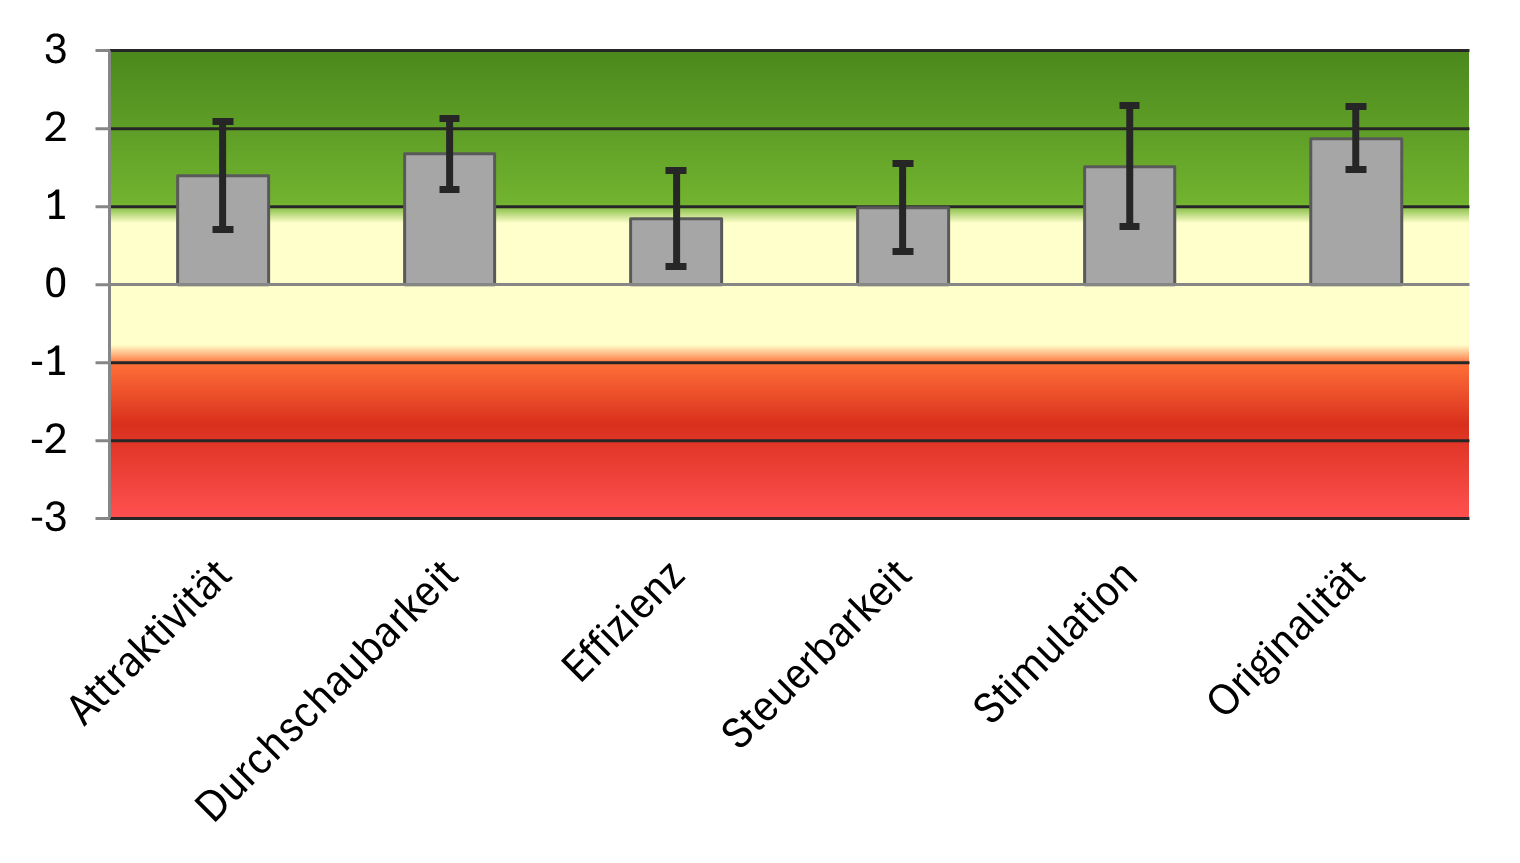
\includegraphics{images/Results/UEQ-Item.png}
 \caption{Ergebnisse UEQ Item Scanning}
 \label{fig:ueqScoreItem}
\end{figure}

\begin{figure}[tbh]
 \centering
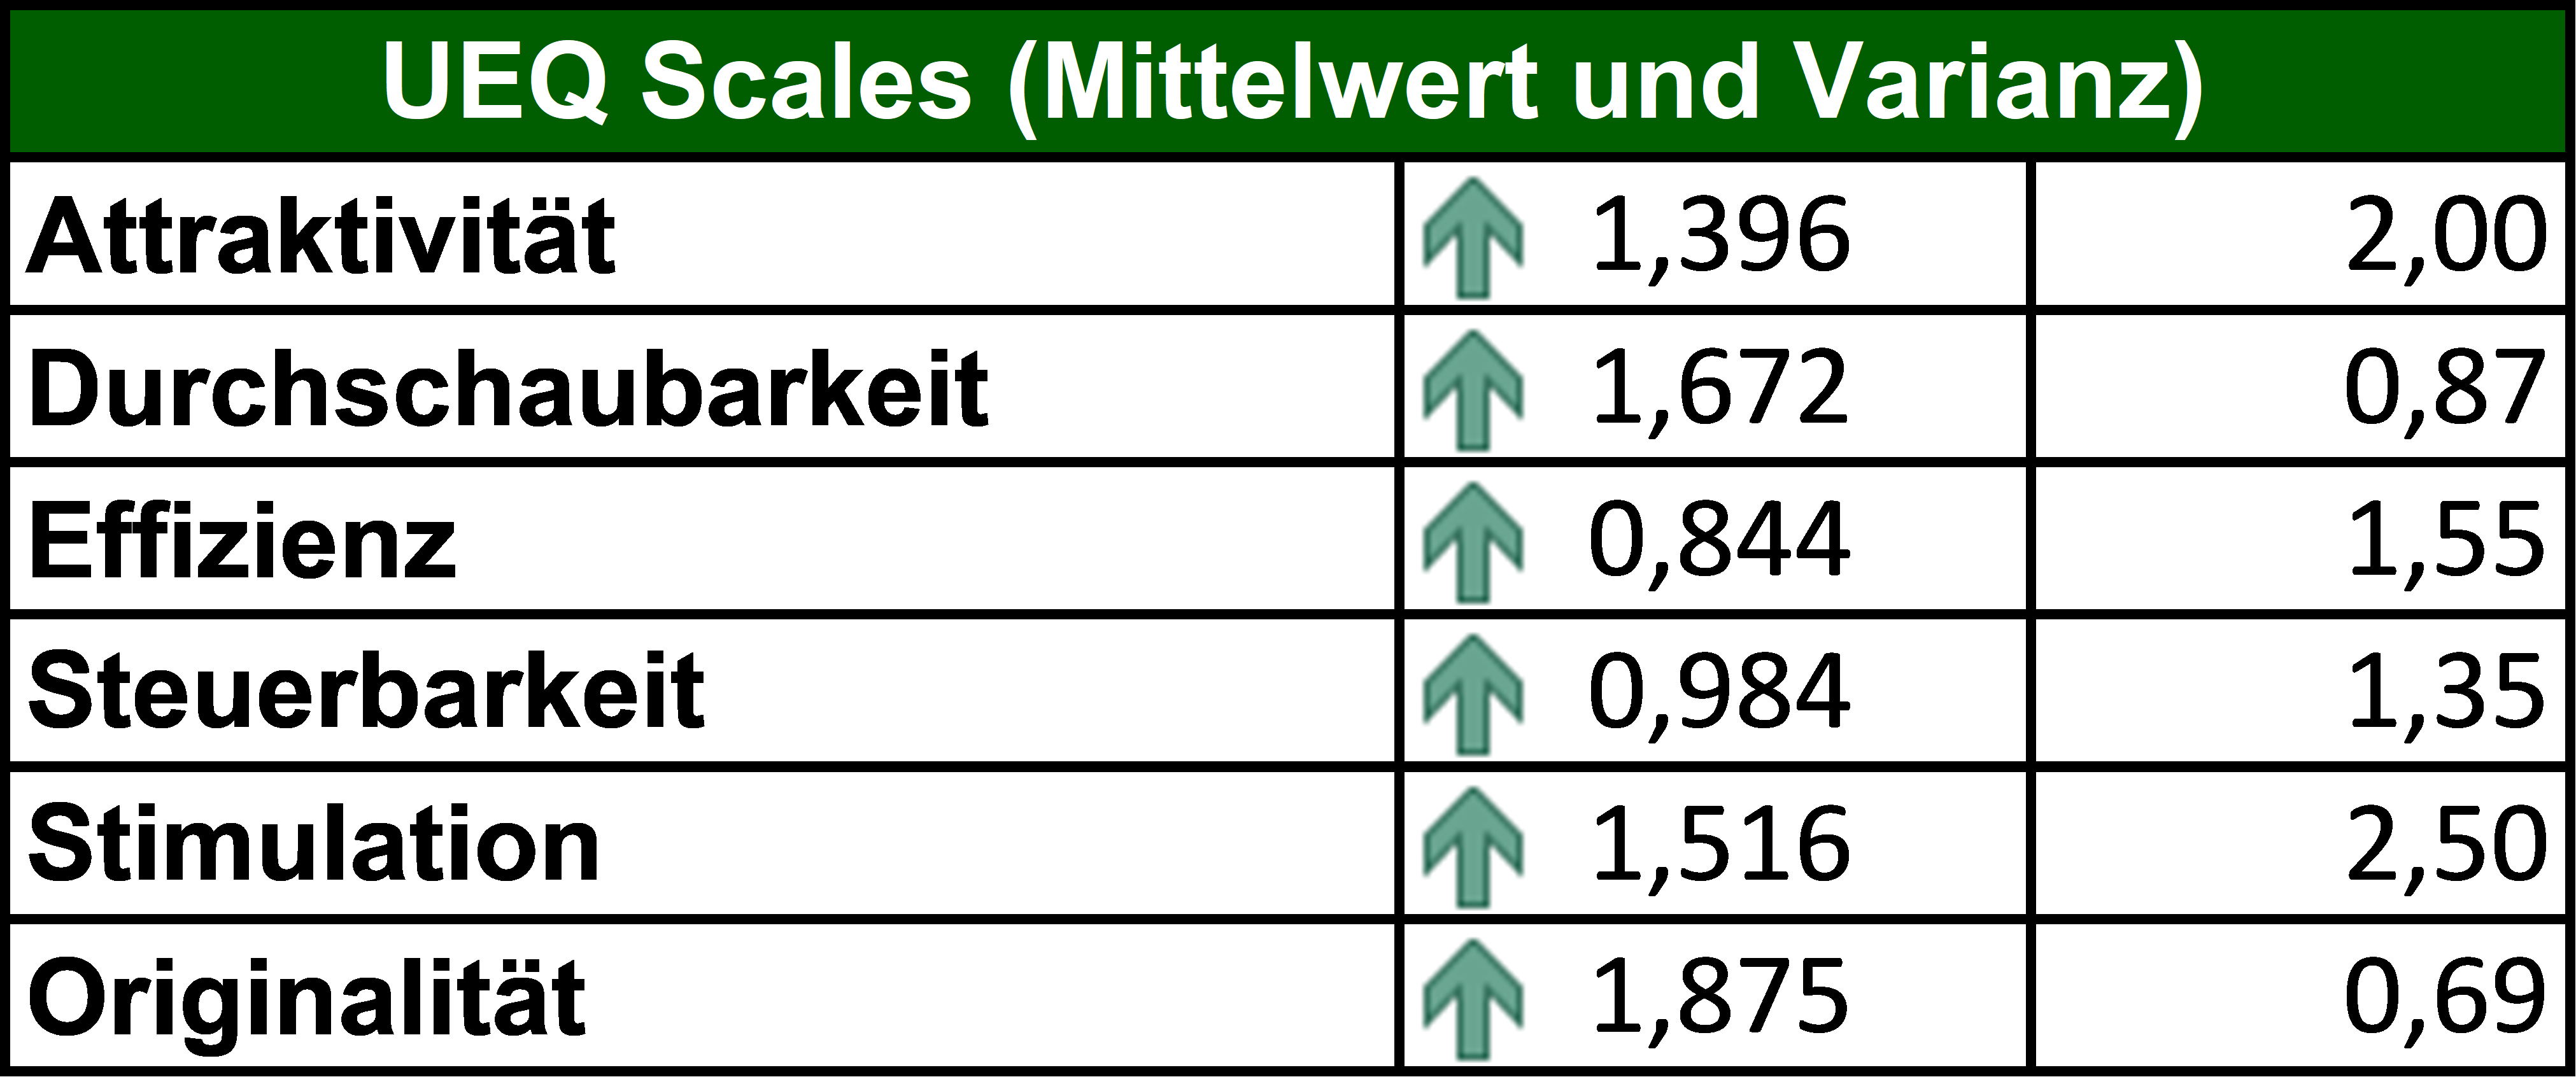
\includegraphics{images/Results/UEQ-Table-Means-Item.png}
 \caption{Ergebnisse UEQ Item Scanning}
 \label{fig:ueqScalesItem}
\end{figure}

\begin{figure}[tbh]
 \centering
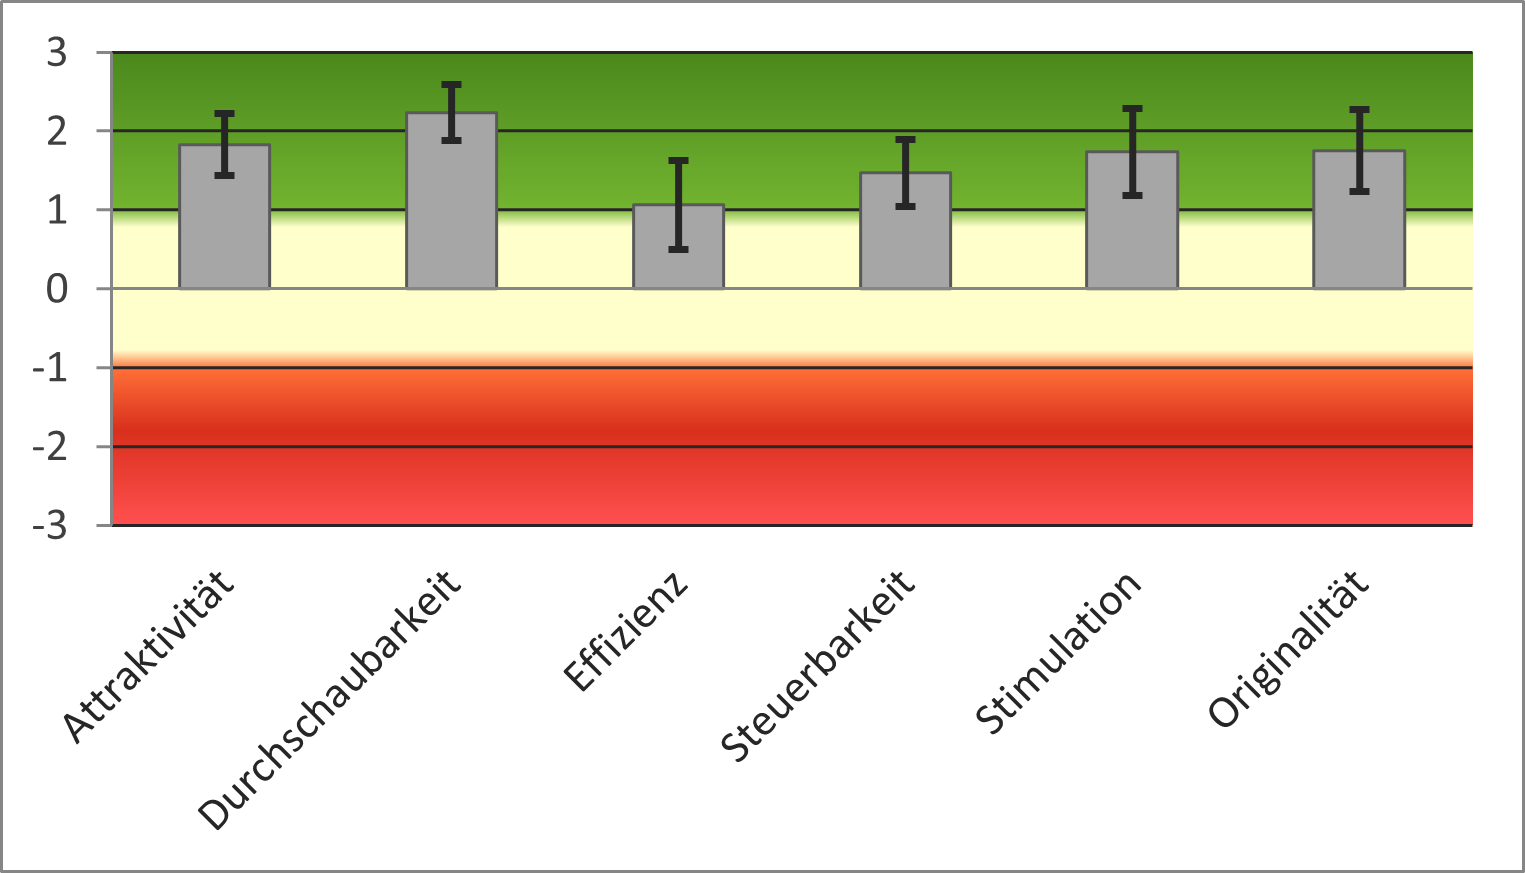
\includegraphics{images/Results/UEQ-Cartesian.png}
 \caption{Ergebnisse UEQ Cartesian Scanning}
 \label{fig:ueqScoreCartesian}
\end{figure}

\begin{figure}[tbh]
 \centering
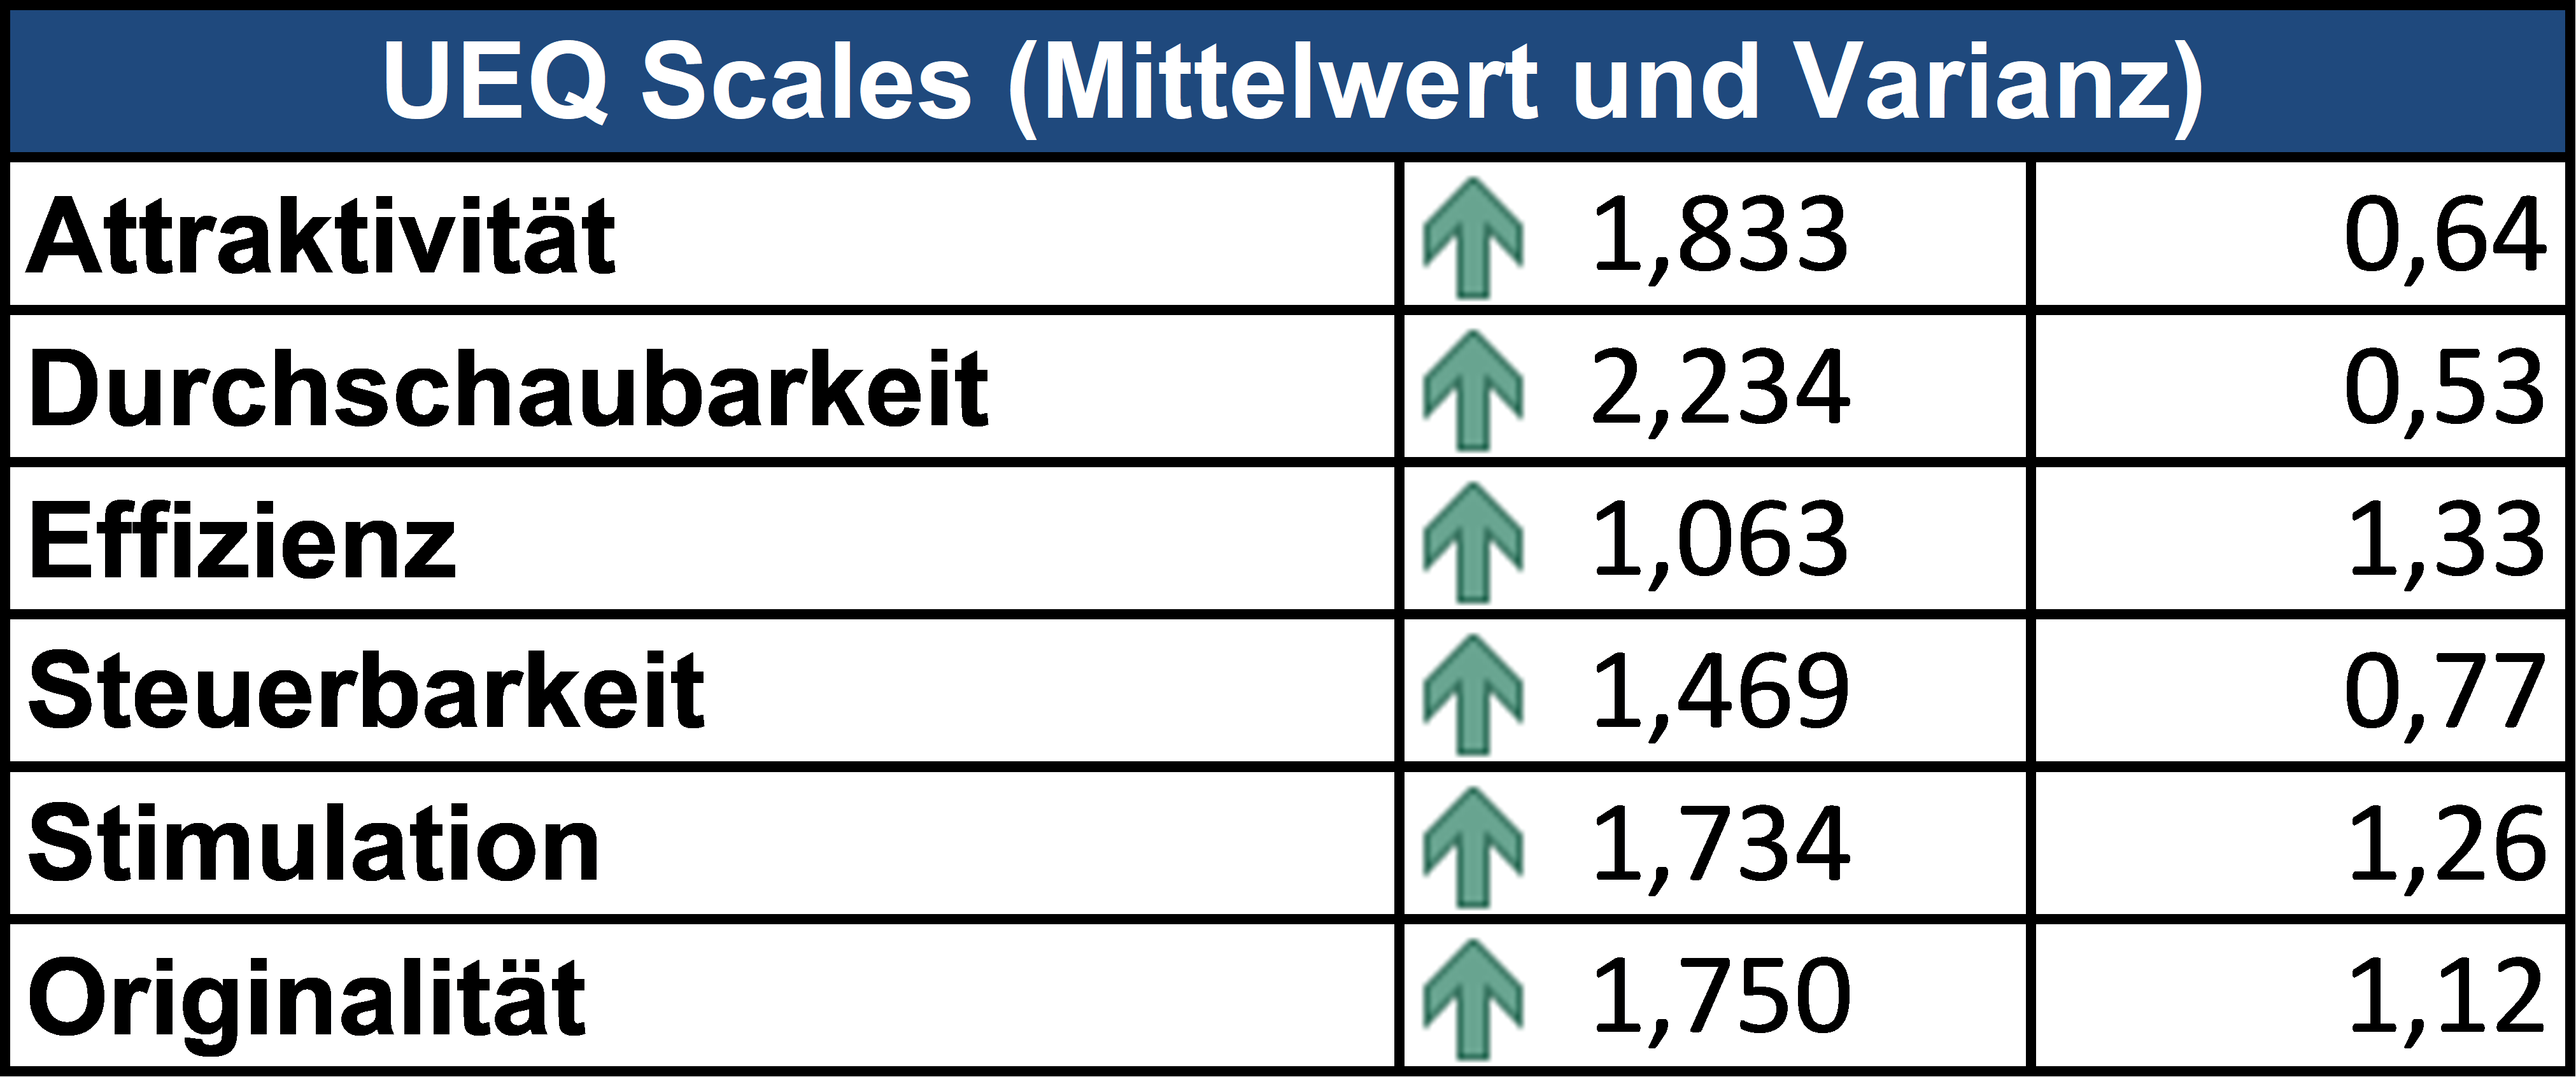
\includegraphics{images/Results/UEQ-Table-Means-Cartesian.png}
 \caption{Ergebnisse UEQ Cartesian Scanning}
 \label{fig:ueqScalesCartesian}
\end{figure}

\subsection{SUS}

\begin{figure}[tbh]
 \centering
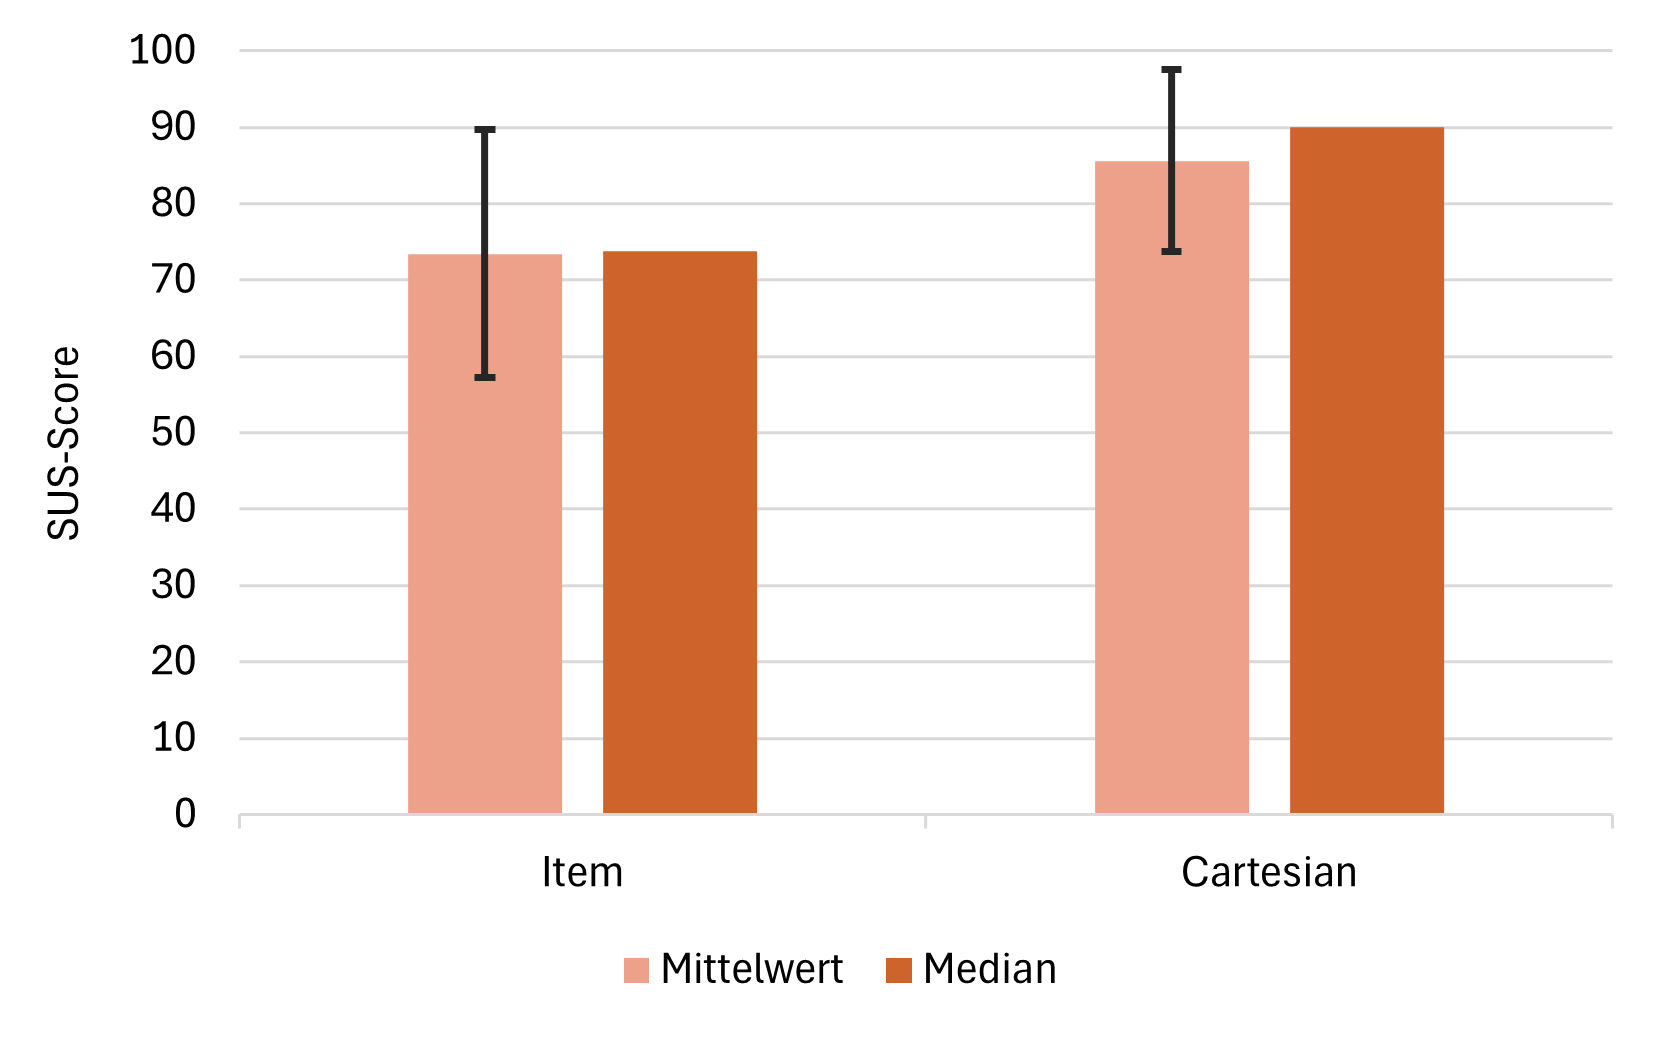
\includegraphics{images/Results/SUS-Scores.png}
 \caption{Ergebnisse SUS}
 \label{fig:resultsSUS}
\end{figure}

\begin{figure}[tbh]
 \centering
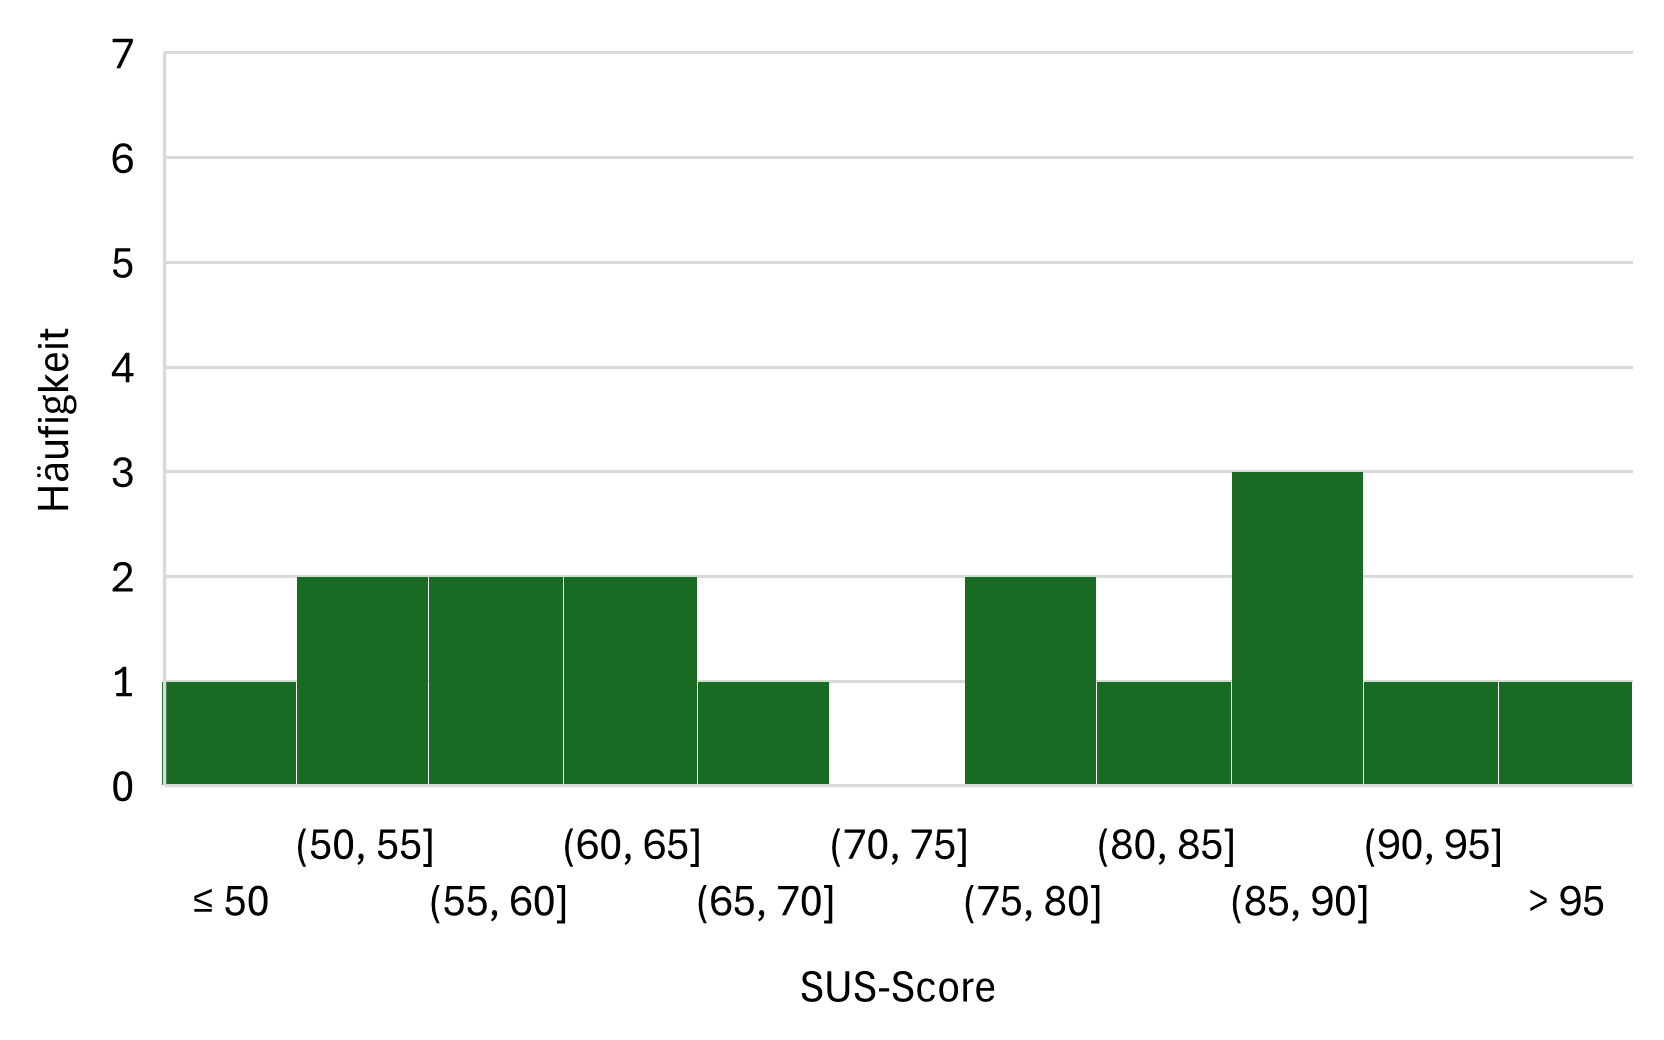
\includegraphics{images/Results/Histogramm-SUS-Item.png}
 \caption{Histogramm SUS Item Scanning}
 \label{fig:histoSUSItem}
\end{figure}

\begin{figure}[tbh]
 \centering
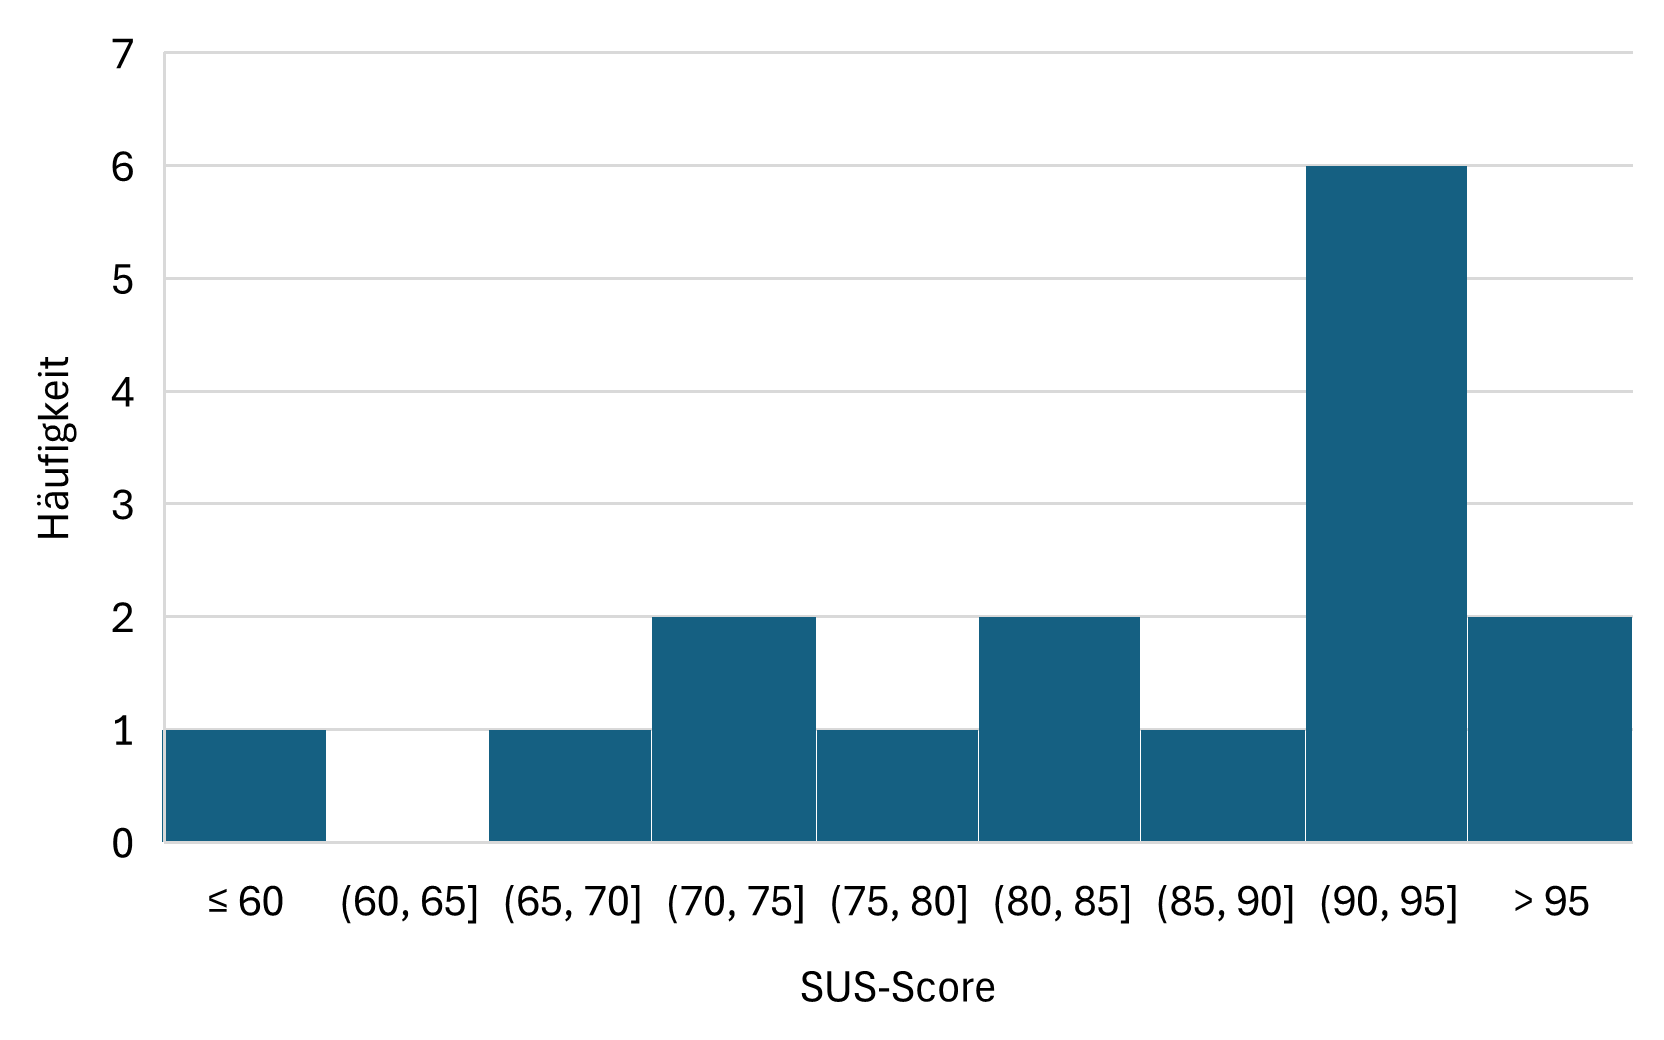
\includegraphics{images/Results/Histogramm-SUS-Cartesian.png}
 \caption{Histogramm SUS Cartesian Scanning}
 \label{fig:histoSUSCartesian}
\end{figure}

\subsection{SSQ} 

\begin{figure}[tbh]
 \centering
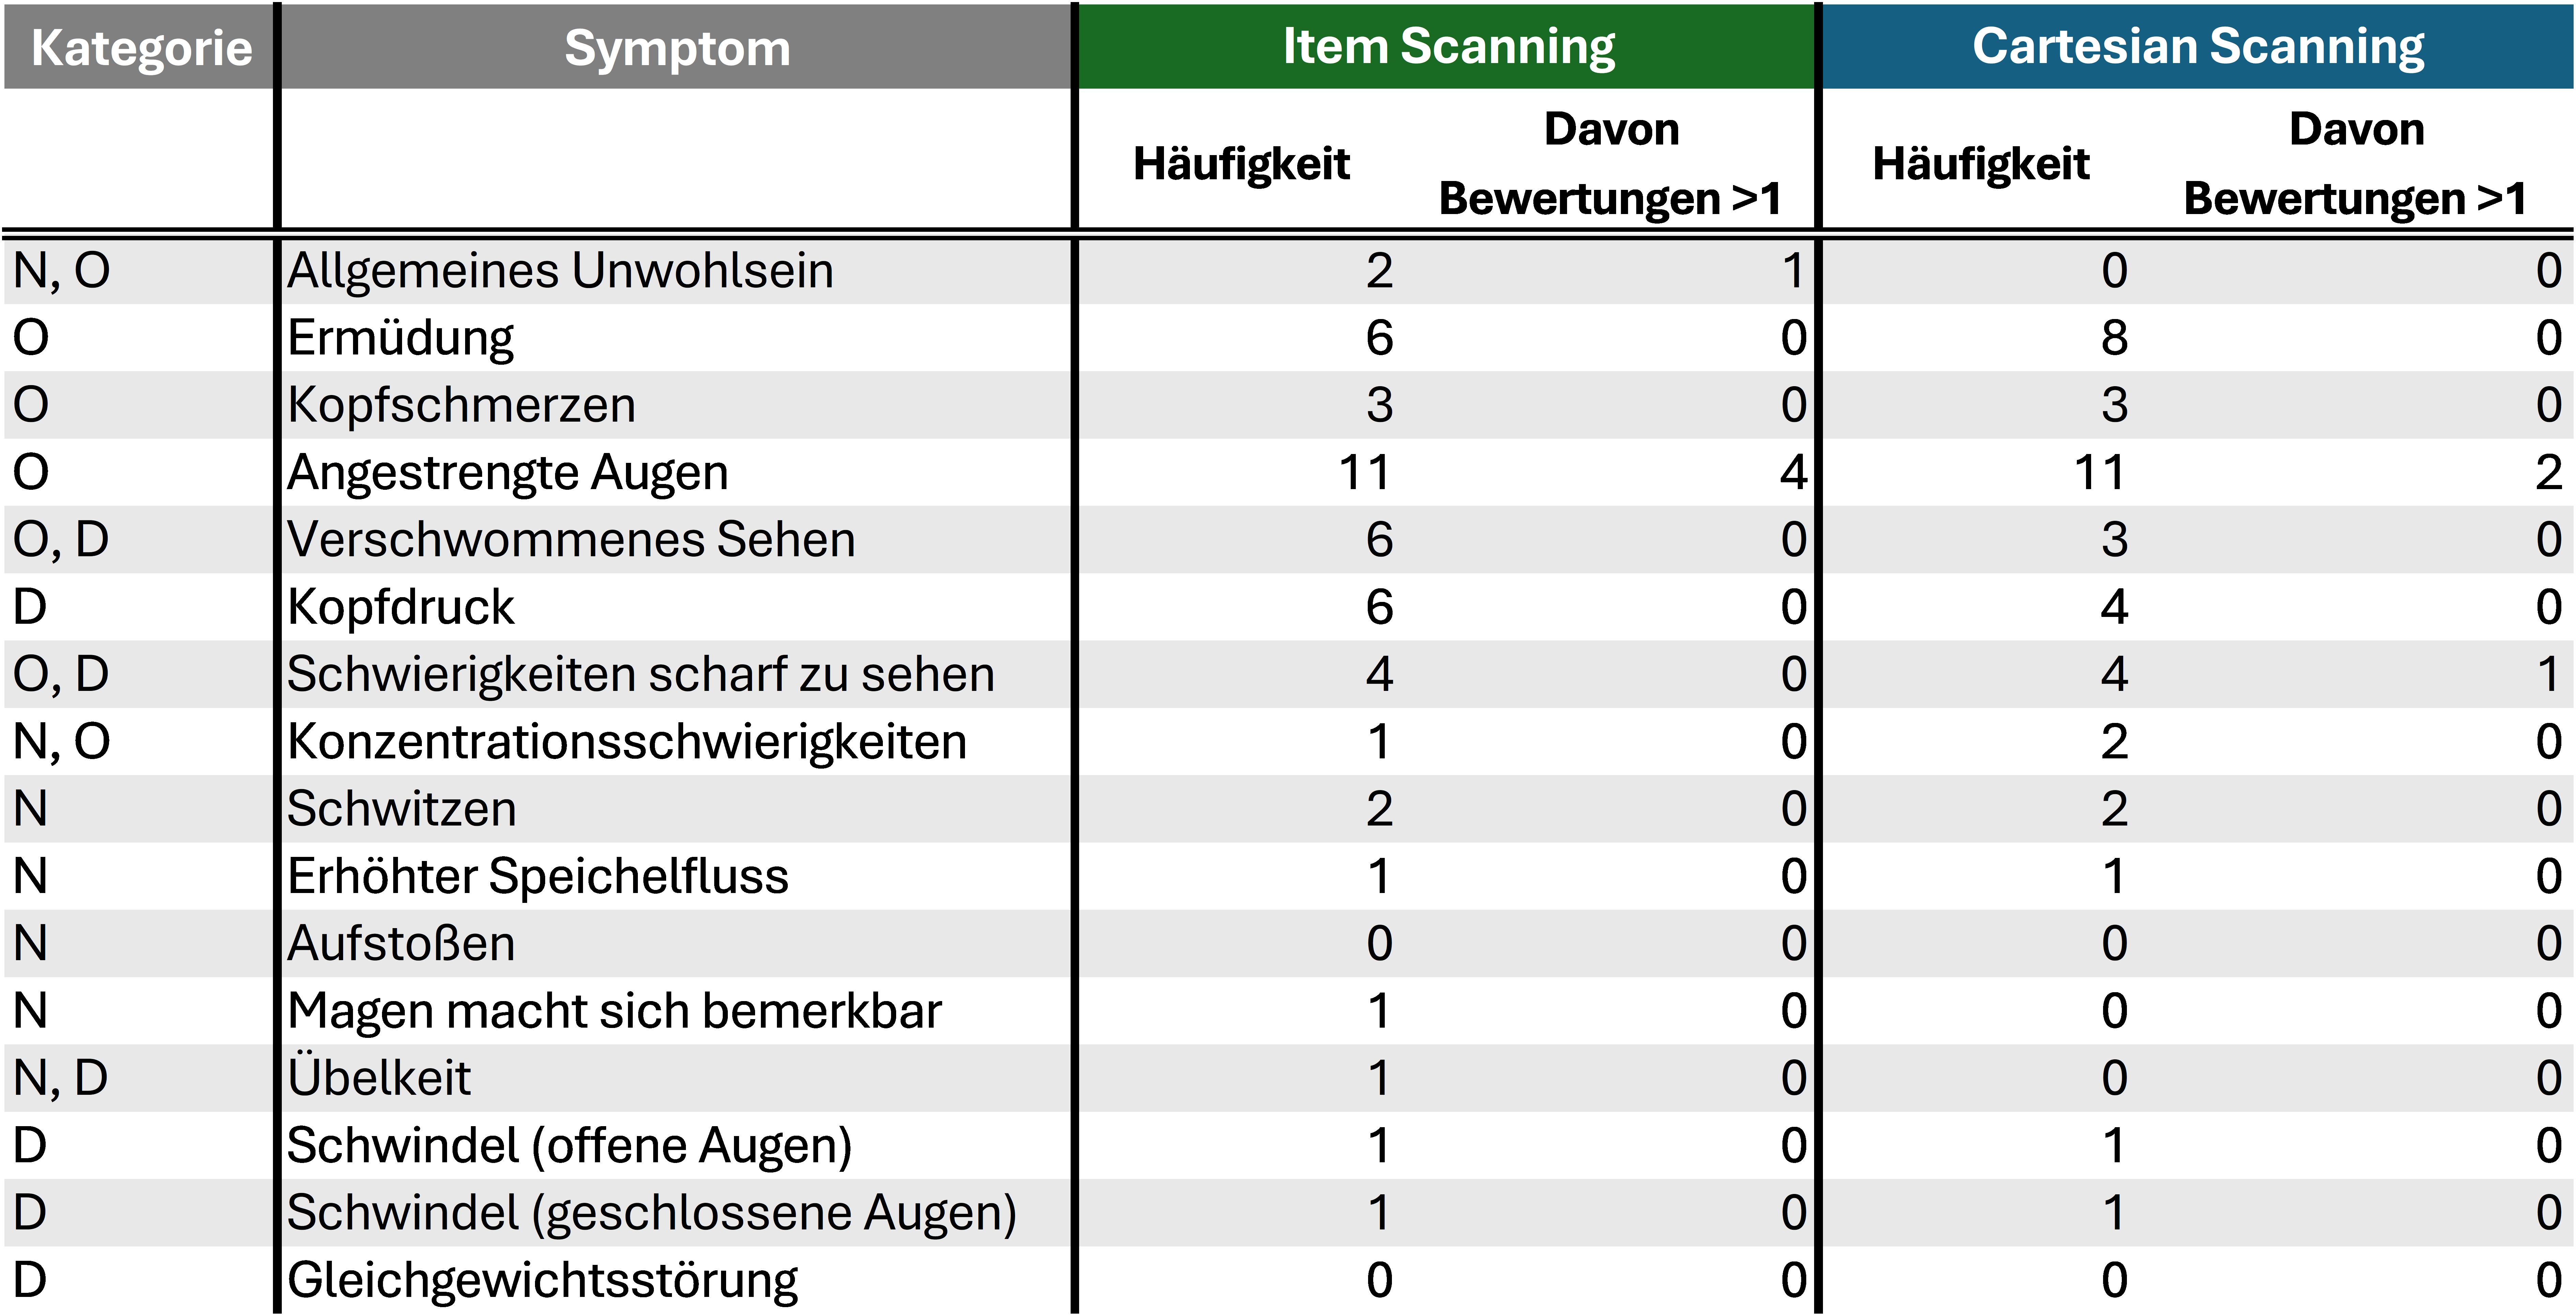
\includegraphics[width=0.95\textwidth]{images/Results/SSQ-Table-2.png}
 \caption{Häufigkeit der Symptome}
 \label{fig:tableSymptomsSSQ}
\end{figure}

\begin{figure}[tbh]
 \centering
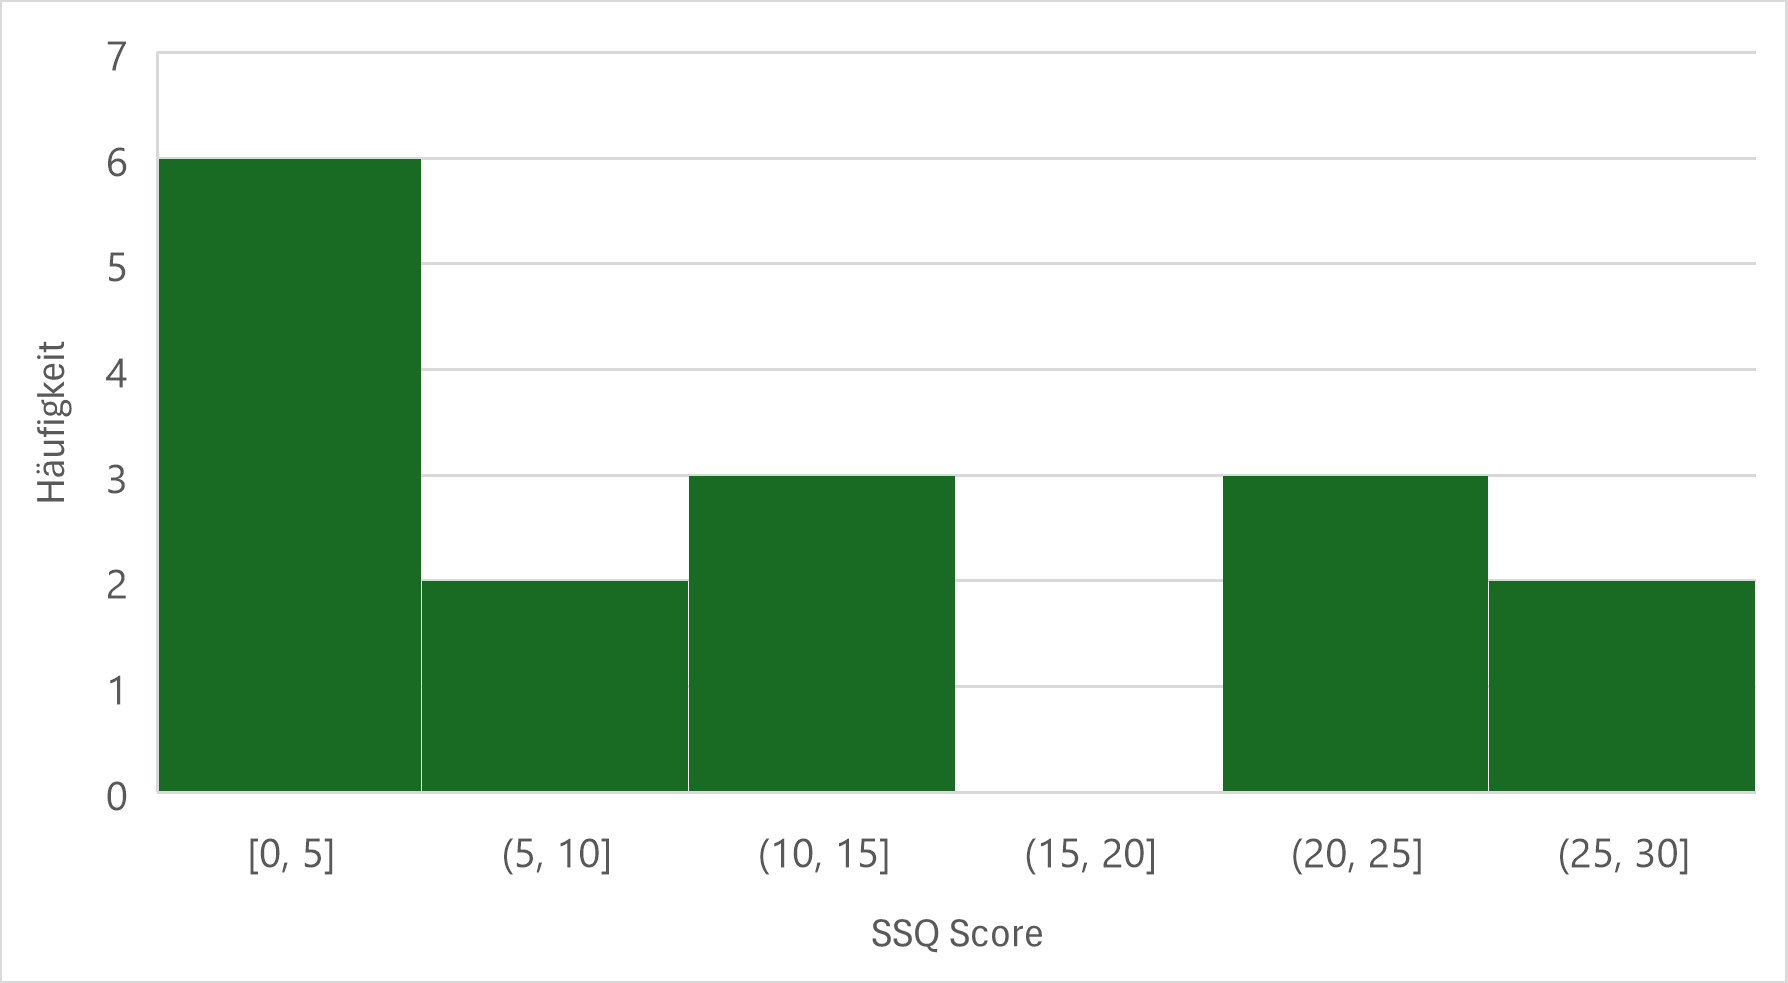
\includegraphics{images/Results/Histogramm-SSQScores-Item.png}
 \caption{Histogramm SSQ Item Scanning}
 \label{fig:histoSSQItem}
\end{figure}

\begin{figure}[tbh]
 \centering
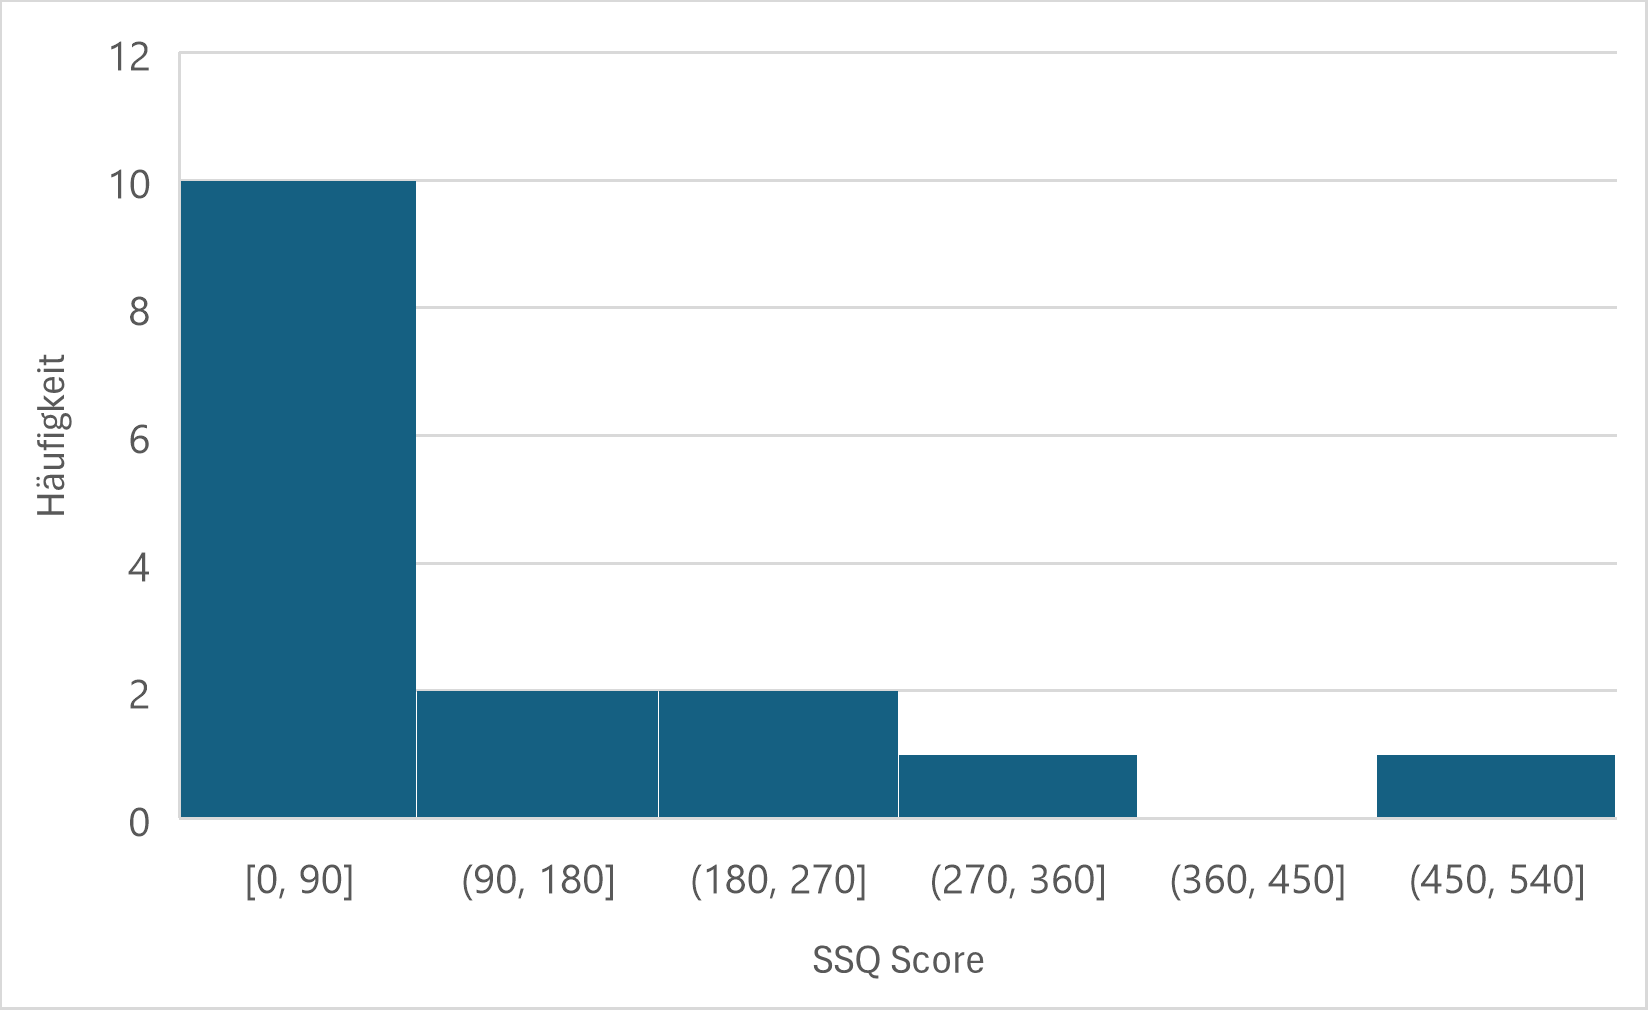
\includegraphics{images/Results/Histogramm-SSQScores-Cartesian.png}
 \caption{Histogramm SSQ Cartesian Scanning}
 \label{fig:histoSSQCartesain}
\end{figure}

\begin{figure}[tbh]
 \centering
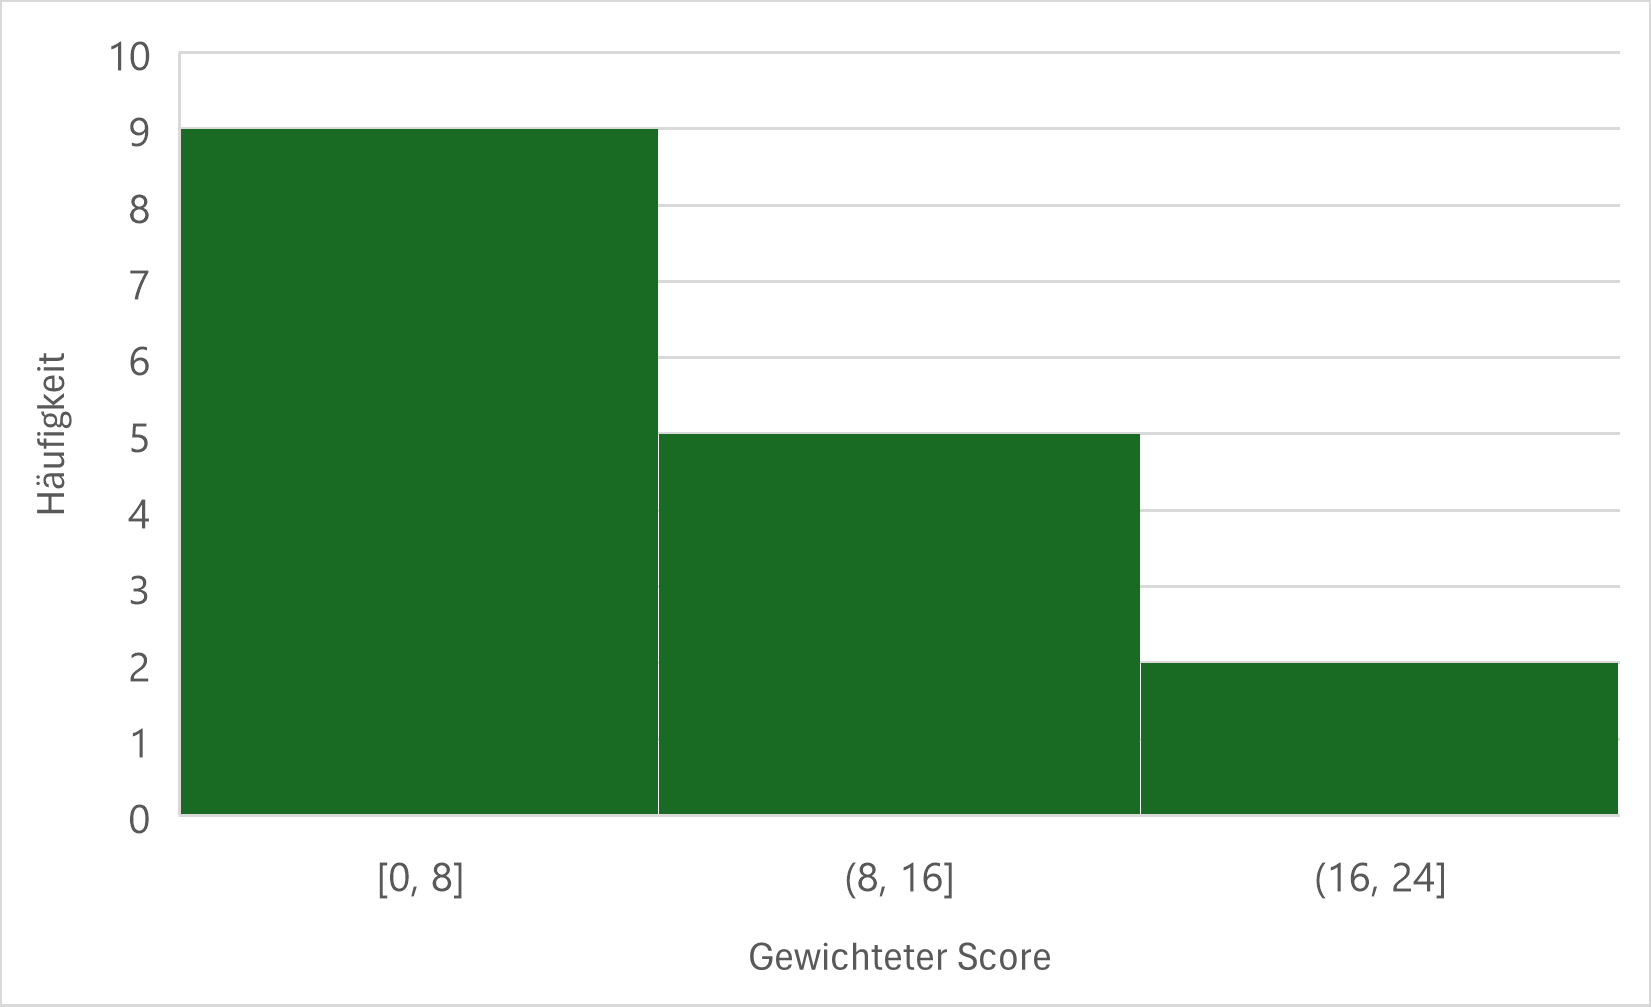
\includegraphics{images/Results/Histogramm-Nausea-Scale-Item.png}
 \caption{Histogramm Nausea Item Scanning}
 \label{fig:histoNauseaItem}
\end{figure}

\begin{figure}[tbh]
 \centering
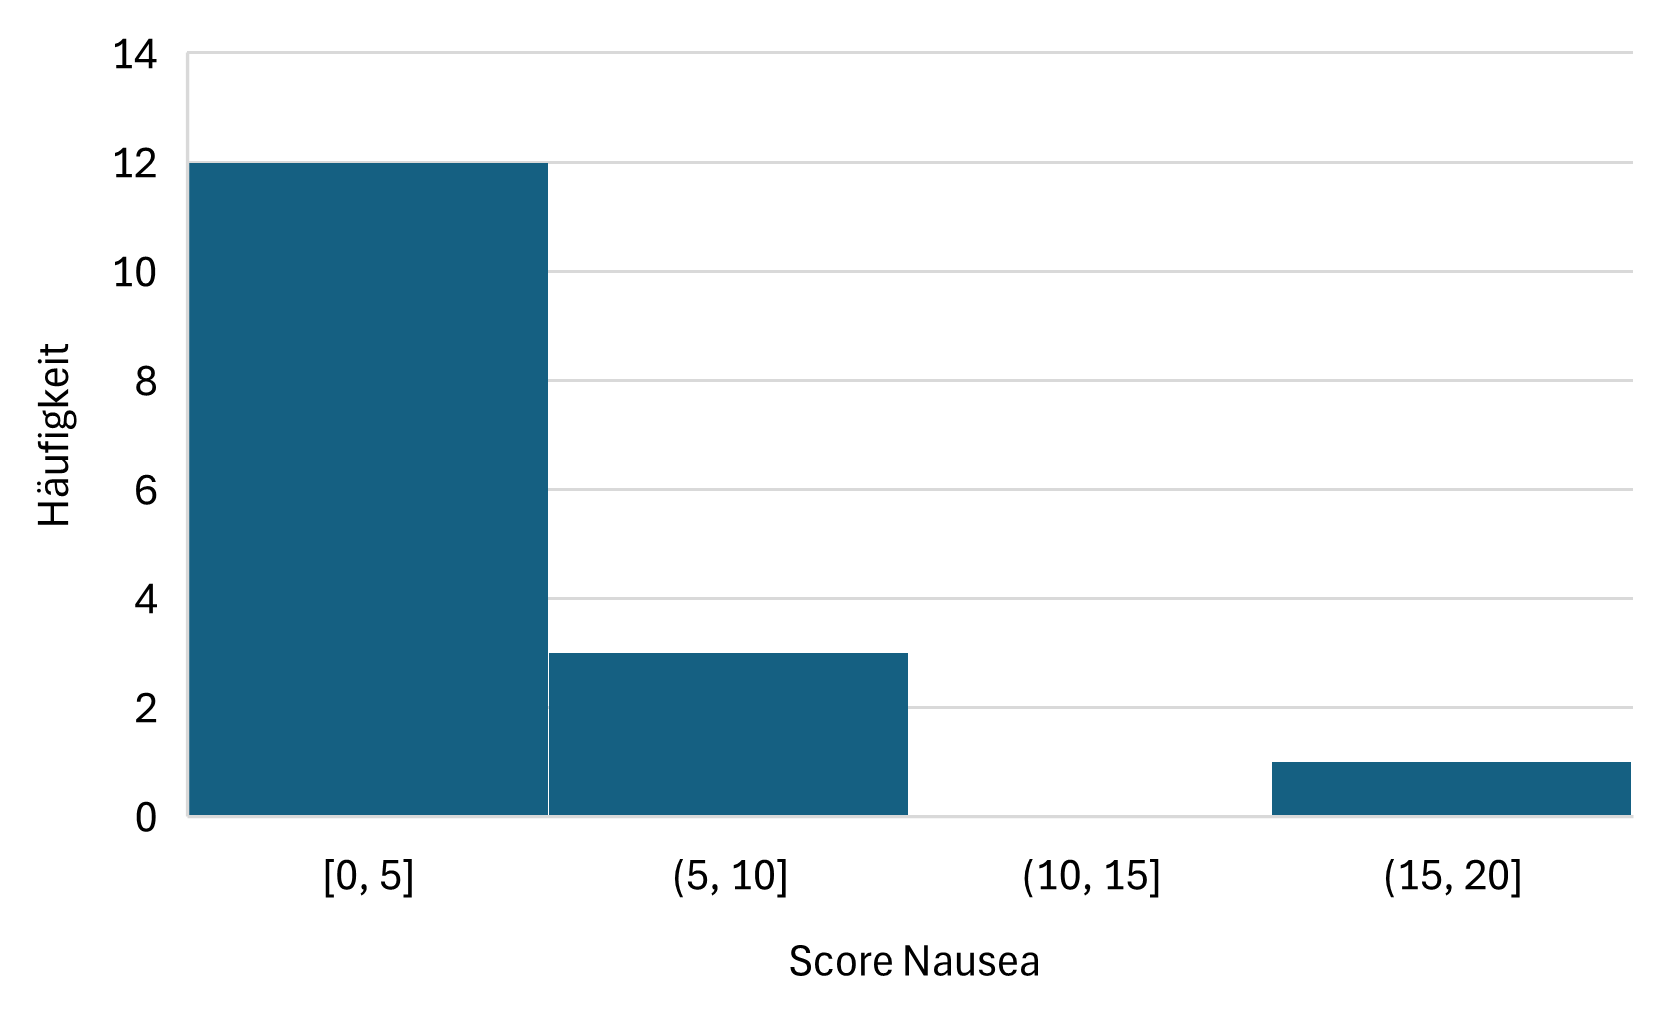
\includegraphics{images/Results/Histogramm-Nausea-Scale-Cartesian.png}
 \caption{Histogramm Nausea Cartesian Scanning}
 \label{fig:histoNauseaCartesian}
\end{figure}

\begin{figure}[tbh]
 \centering
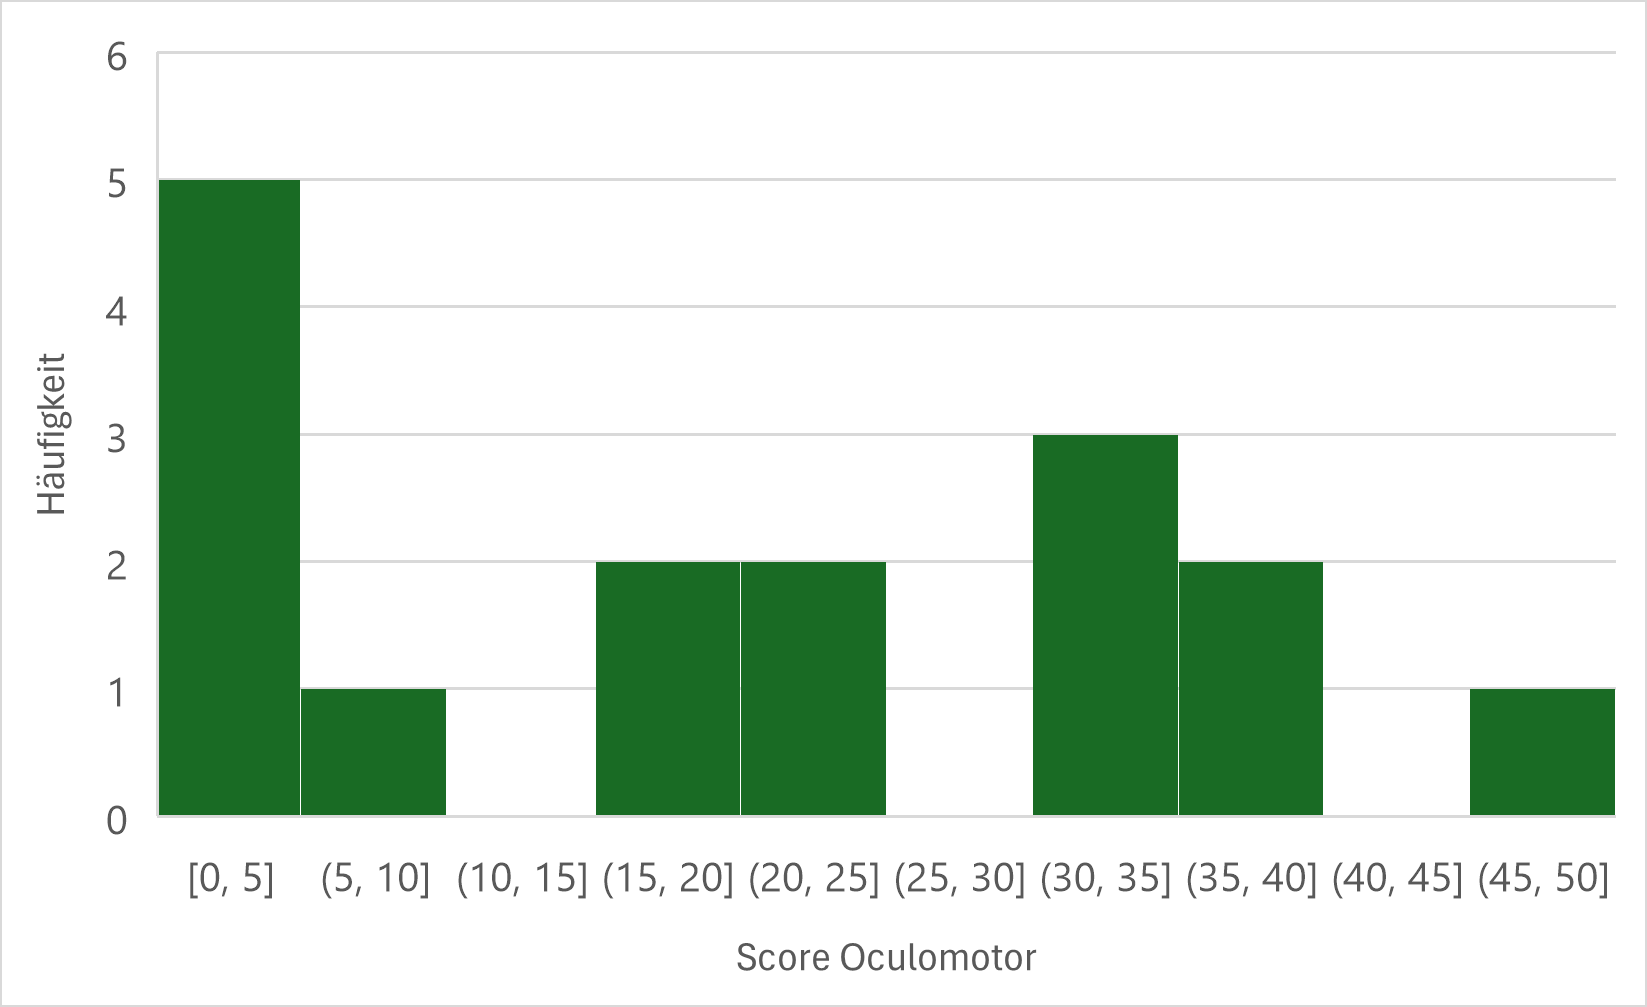
\includegraphics{images/Results/Histogramm-Oculomotor-Scale-Item.png}
 \caption{Histogramm Oculomotor Item Scanning}
 \label{fig:histoOculomotorItem}
\end{figure}

\begin{figure}[tbh]
 \centering
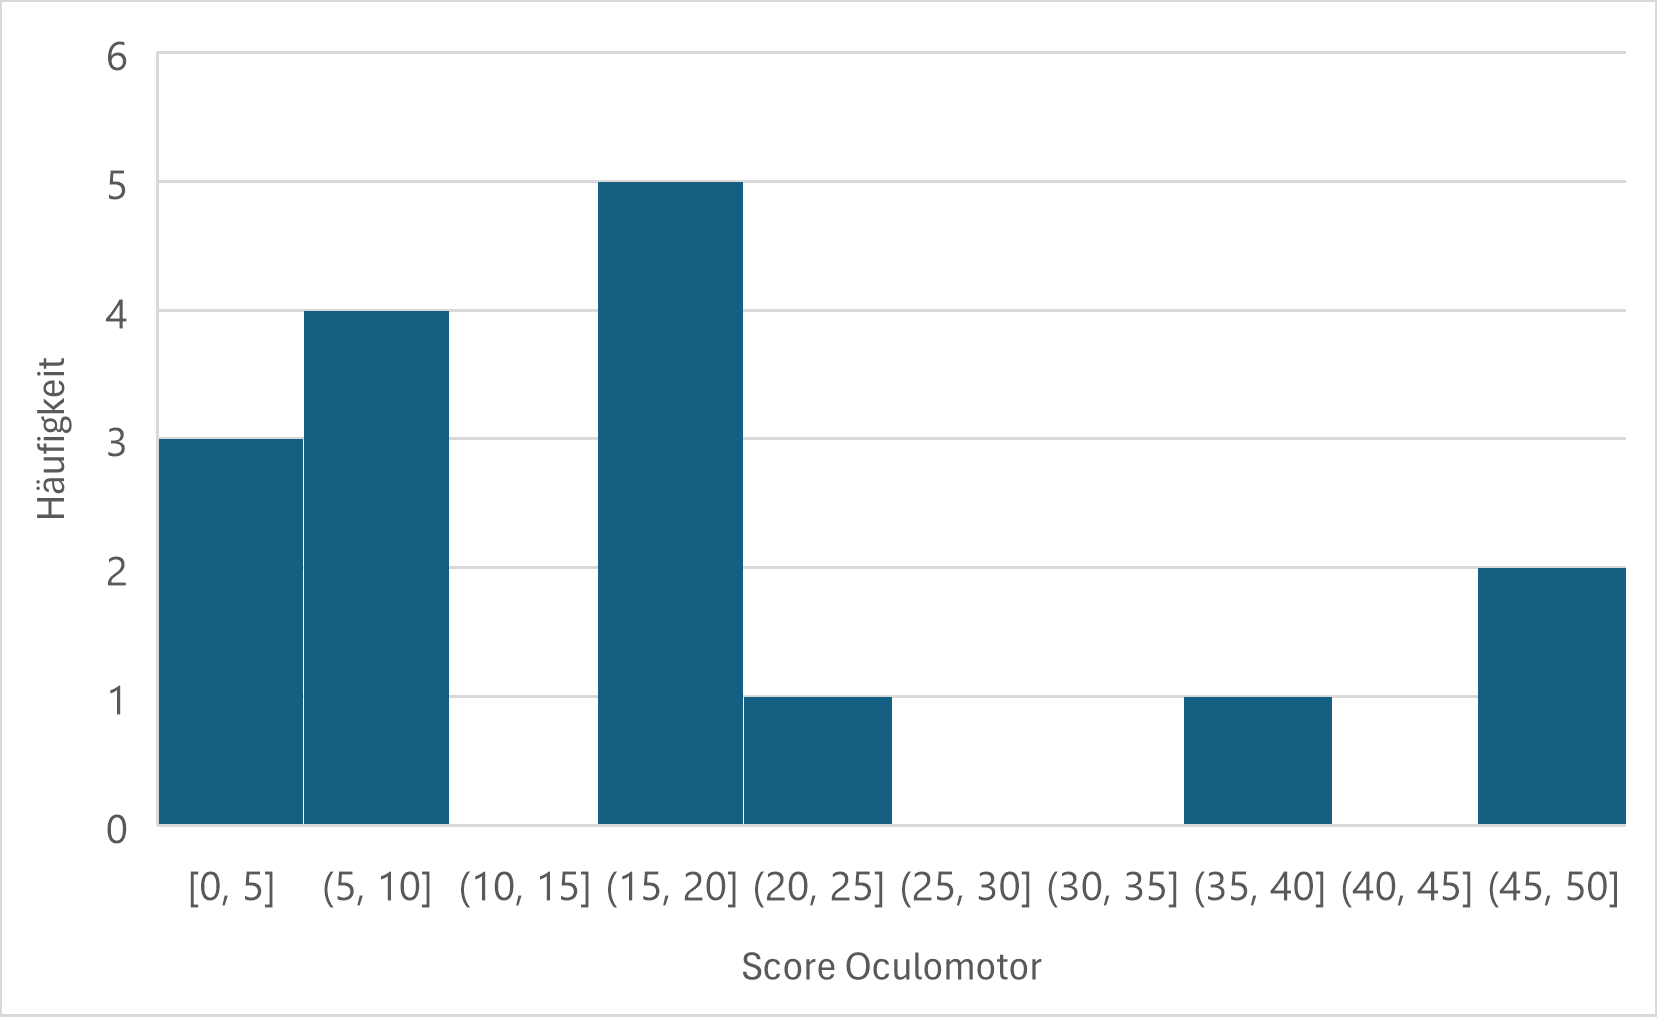
\includegraphics{images/Results/Histogramm-Oculomotor-Scale-Cartesian.png}
 \caption{Histogramm Oculomotor Cartesian Scanning}
 \label{fig:histoOculomotorCartesian}
\end{figure}

\begin{figure}[tbh]
 \centering
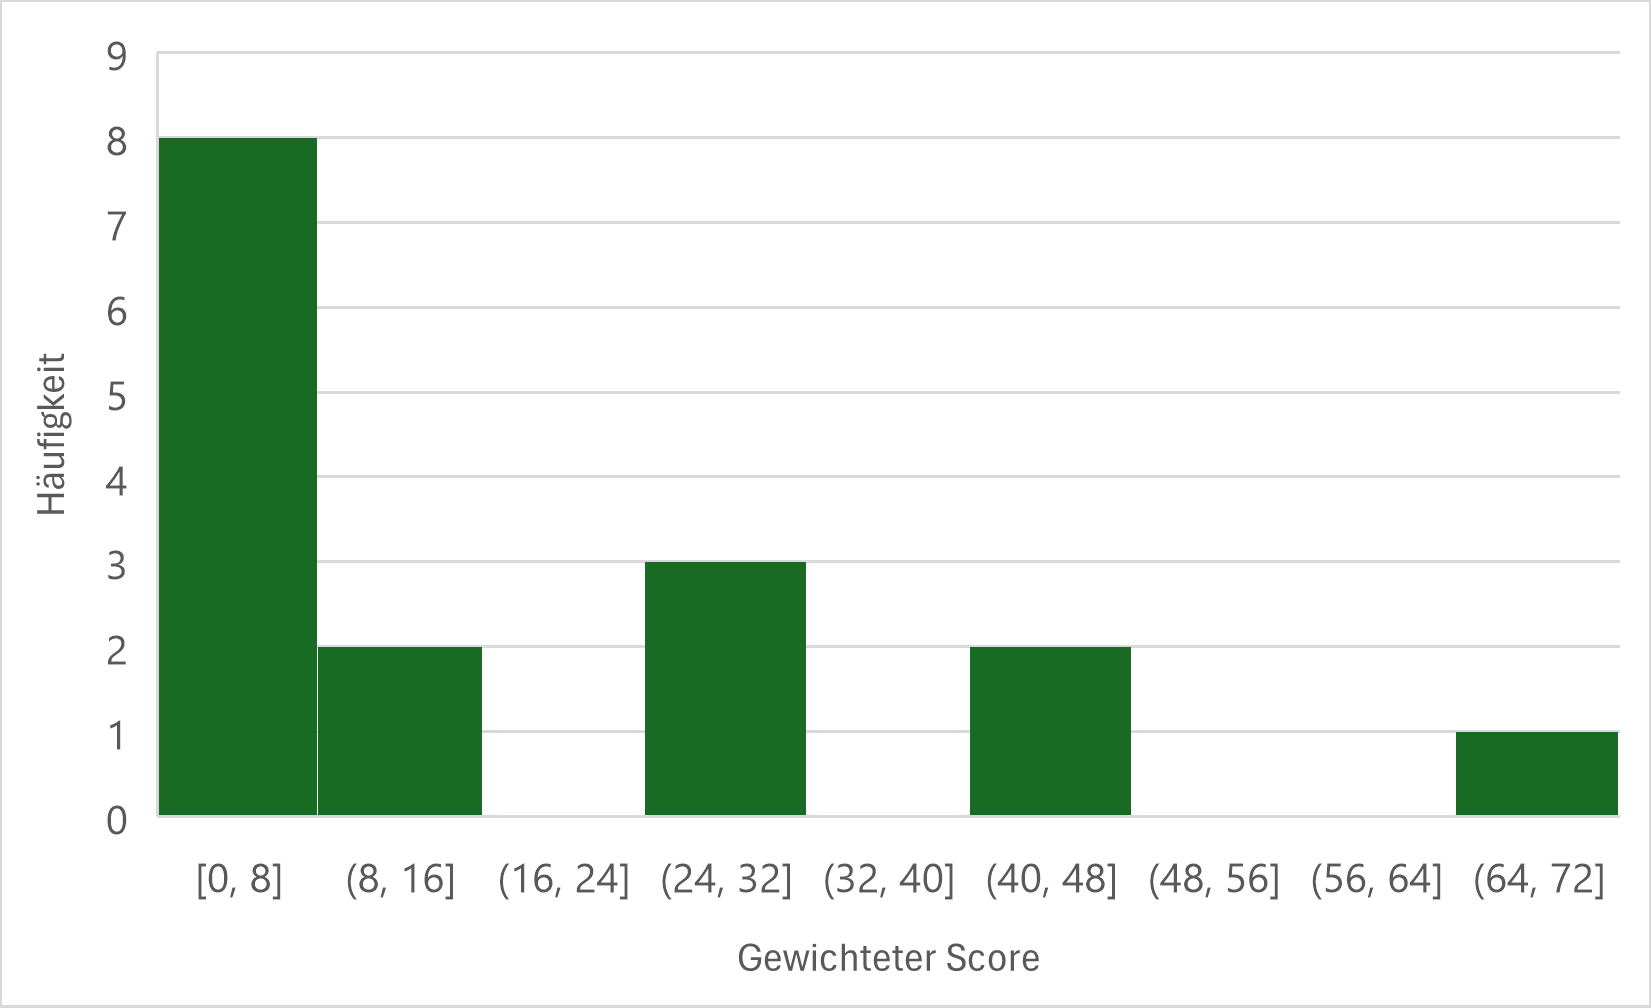
\includegraphics{images/Results/Histogramm-Disorientation-Scale-Item.png}
 \caption{Histogramm Disorientation Item Scanning}
 \label{fig:histoDisorientationItem}
\end{figure}

\begin{figure}[tbh]
 \centering
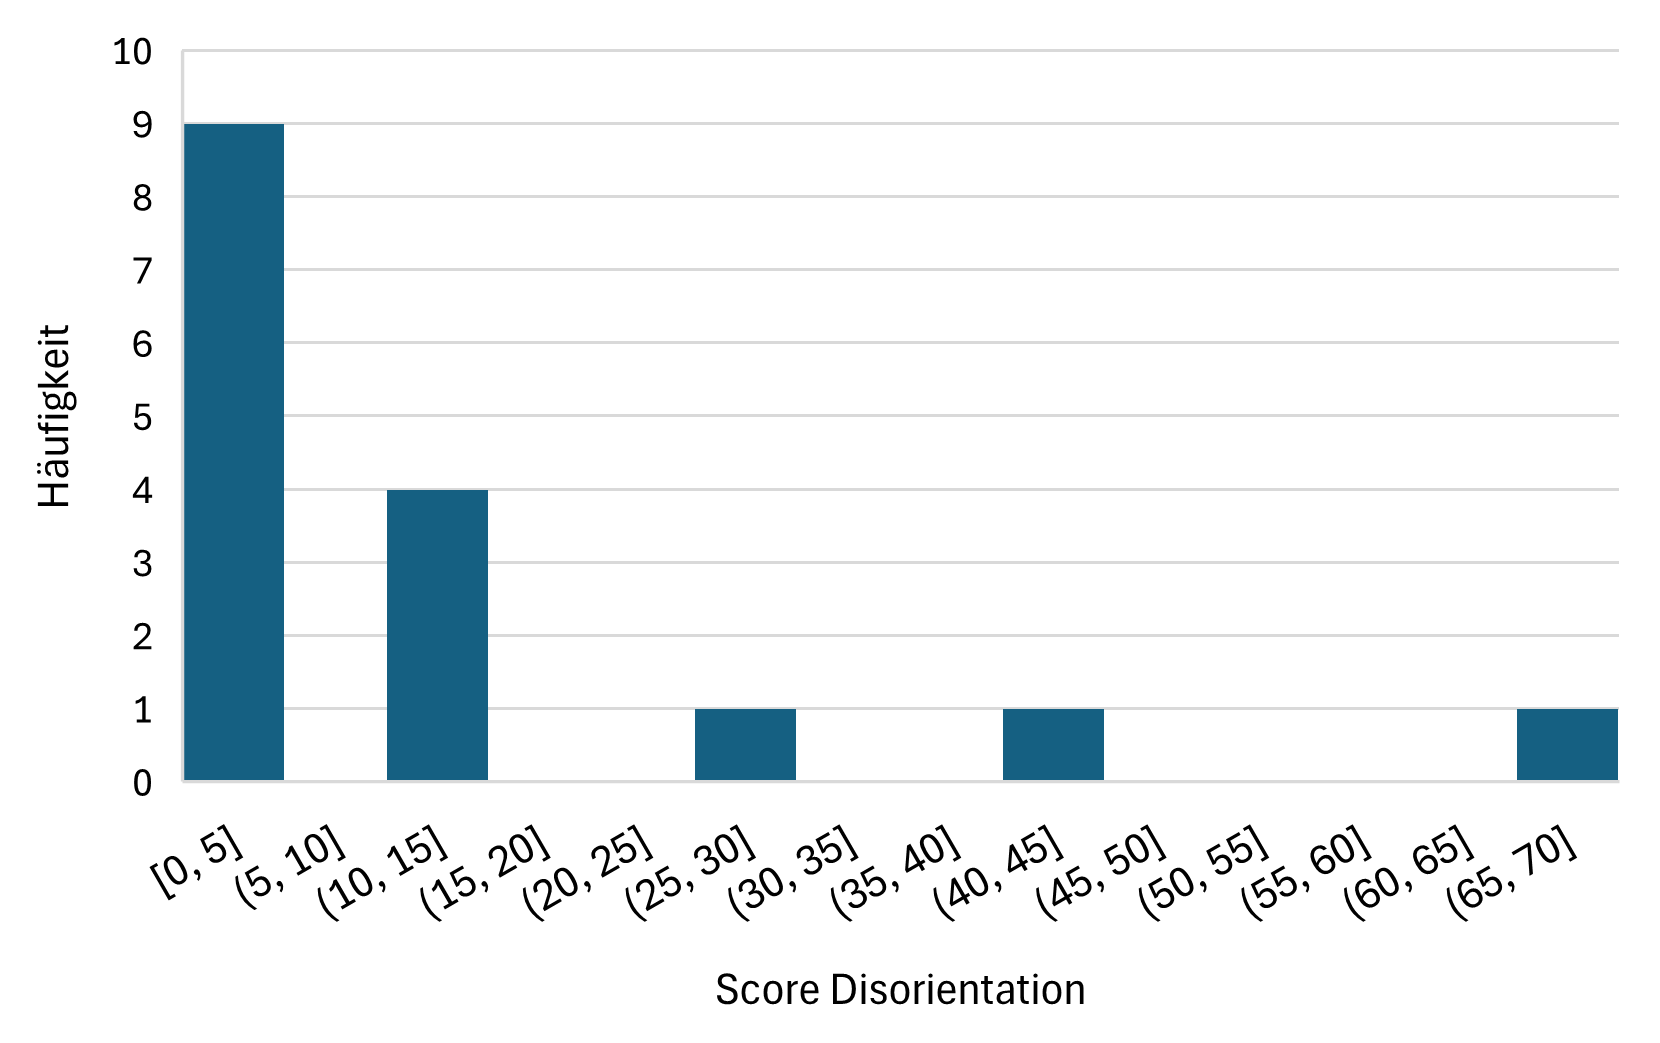
\includegraphics{images/Results/Histogramm-Disorientation-Scale-Cartesian.png}
 \caption{Histogramm Disorientation Cartesian Scanning}
 \label{fig:histoDisorientationCartesian}
\end{figure}

\subsection{Ablenkung/Presence}

\begin{figure}[tbh]
 \centering
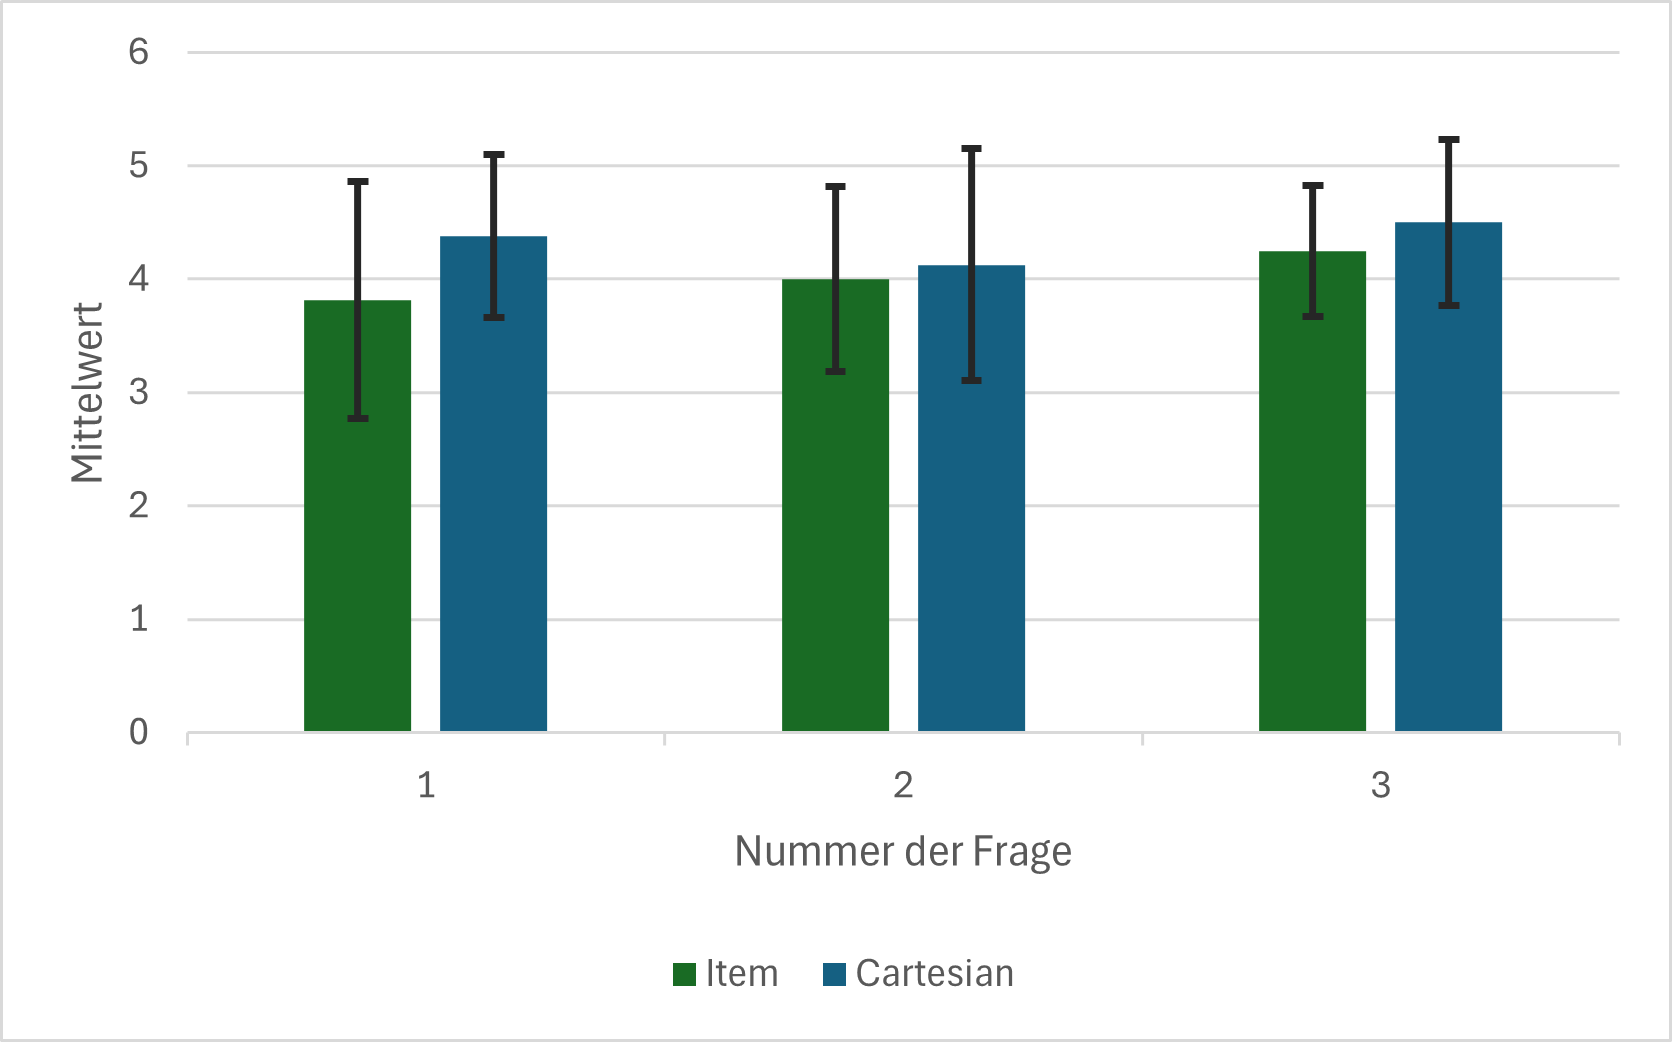
\includegraphics{images/Results/Fragen-zur-Presence-Ablenkung.png}
 \caption{Fragen zur Presence/Ablenkung}
 \label{fig:presence}
\end{figure}

\subsection{Geschwindigkeit und Zkylen}

\begin{figure}[tbh]
 \centering
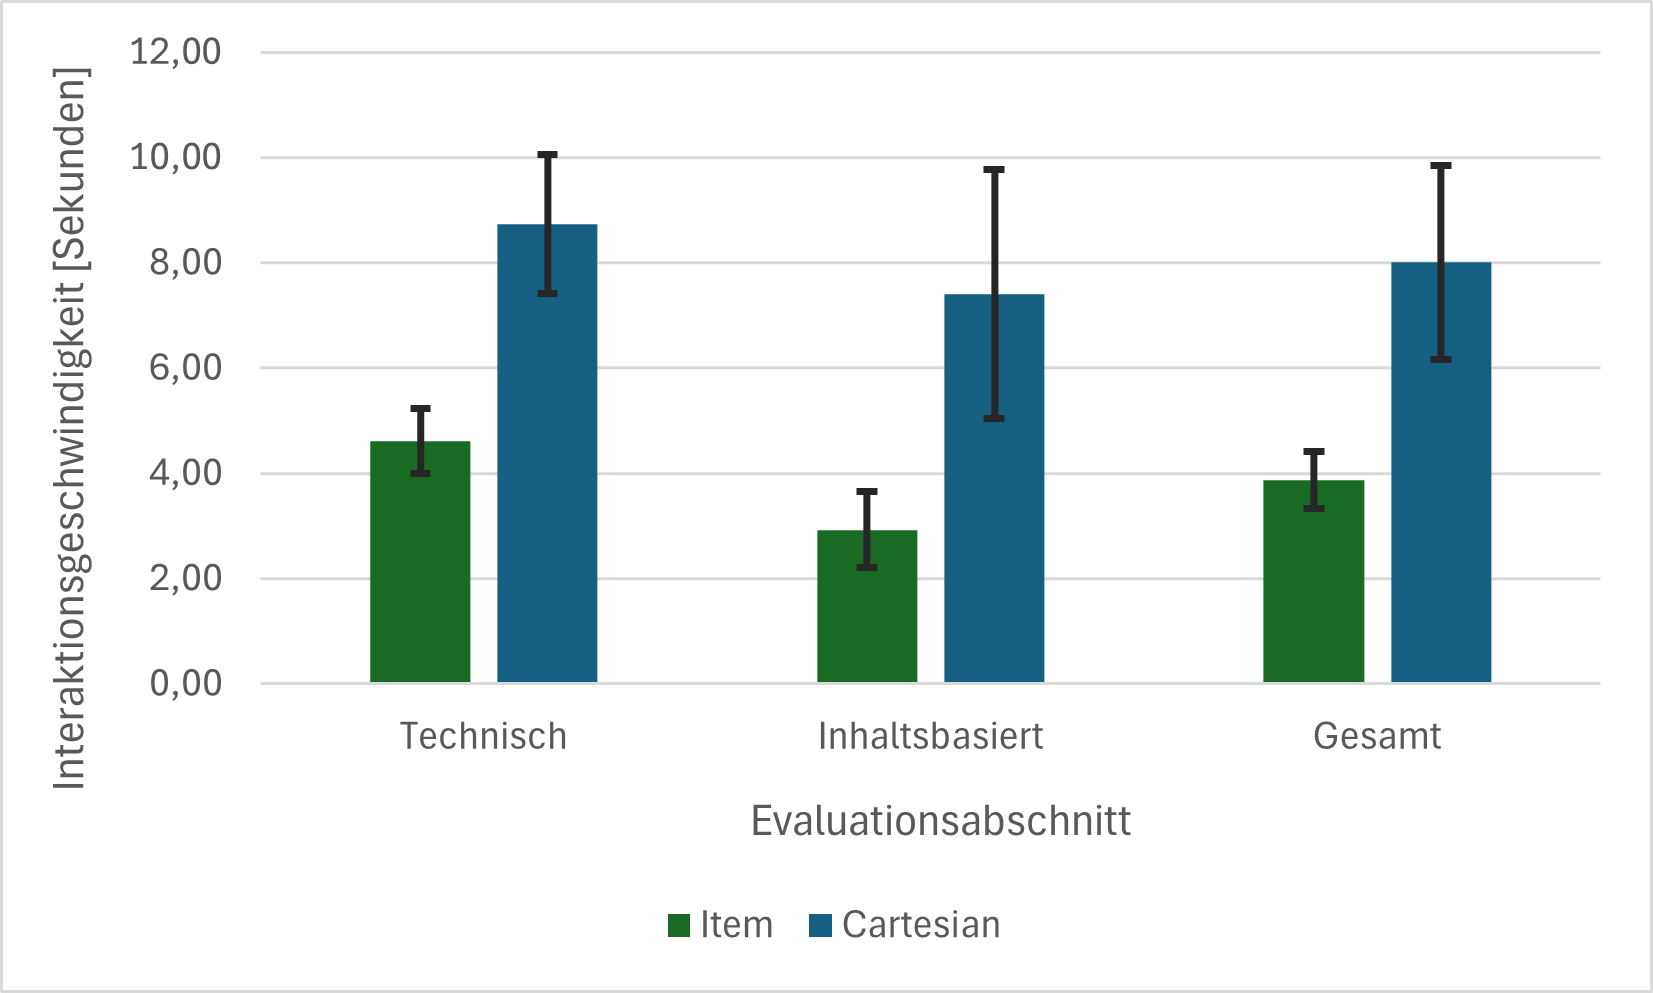
\includegraphics{images/Results/Interaktionsgeschwindigkeiten.png}
 \caption{Interaktionsgeschwindigkeiten}
 \label{fig:Interaktionsgeschwindigkeiten}
\end{figure}

\begin{figure}[tbh]
 \centering
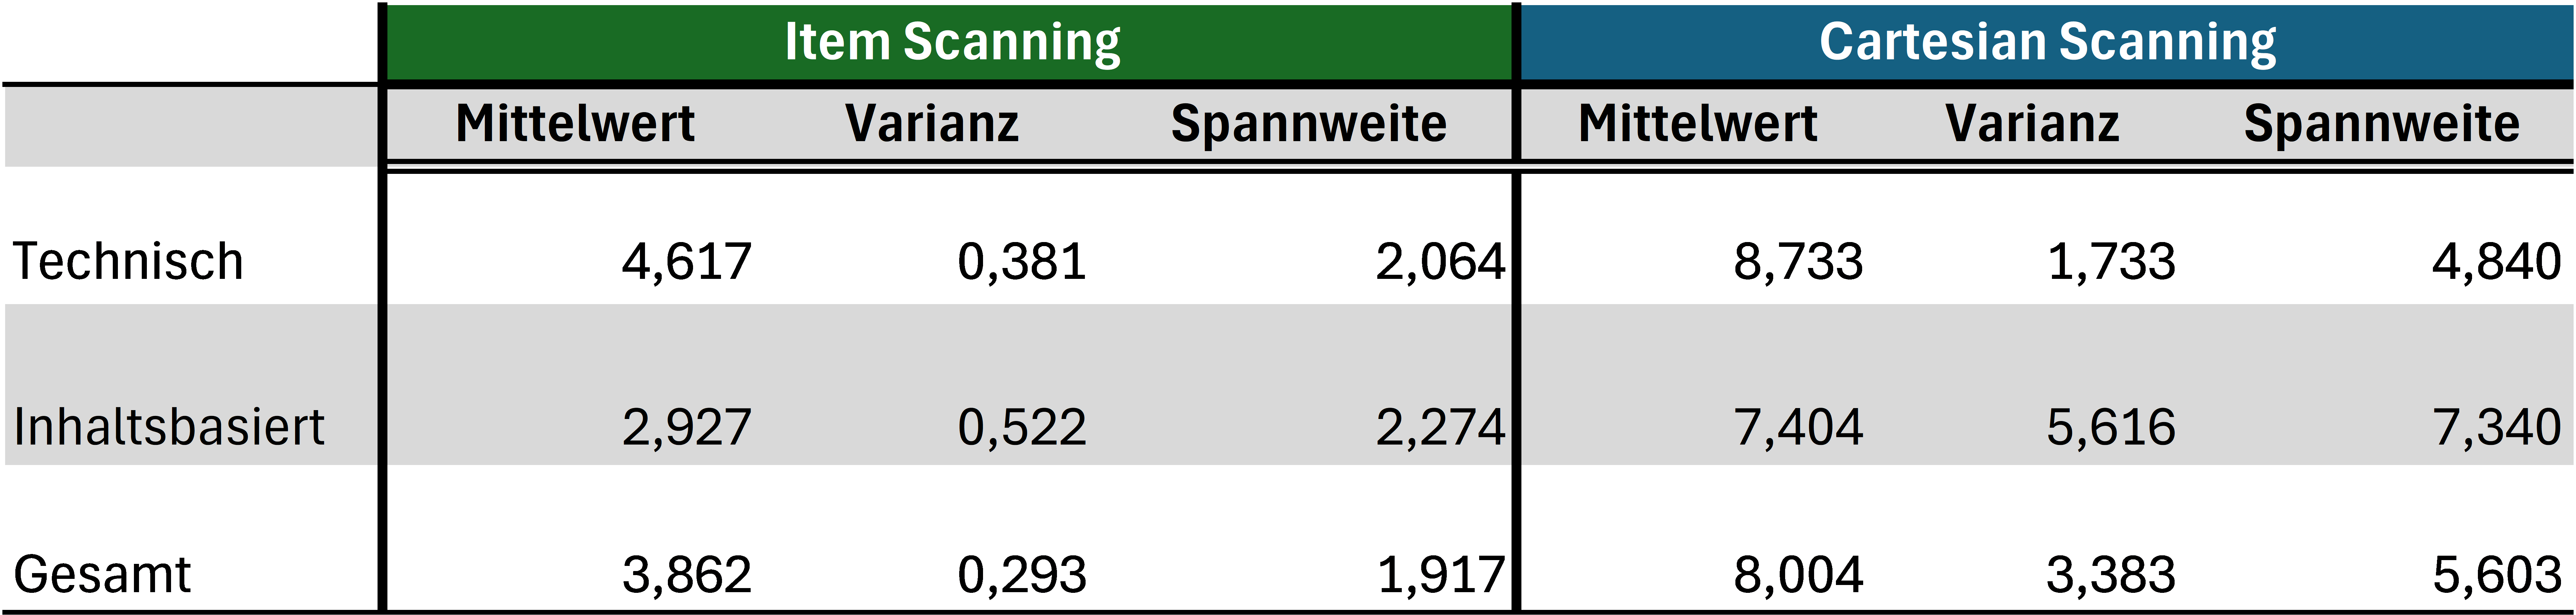
\includegraphics[width=0.95\textwidth]{images/Results/Interaktionsgeschwindigkeiten-Table.png}
 \caption{Interaktionsgeschwindigkeiten Tabelle}
 \label{fig:InteraktionsgeschwindigkeitenTable}
\end{figure}

\begin{figure}[tbh]
 \centering
\includegraphics{images/Results/Benötigte-Zeit-Evaluationsabschnitte.png}
 \caption{Benötigte Zeit}
 \label{fig:zeit}
\end{figure}

\begin{figure}[tbh]
 \centering
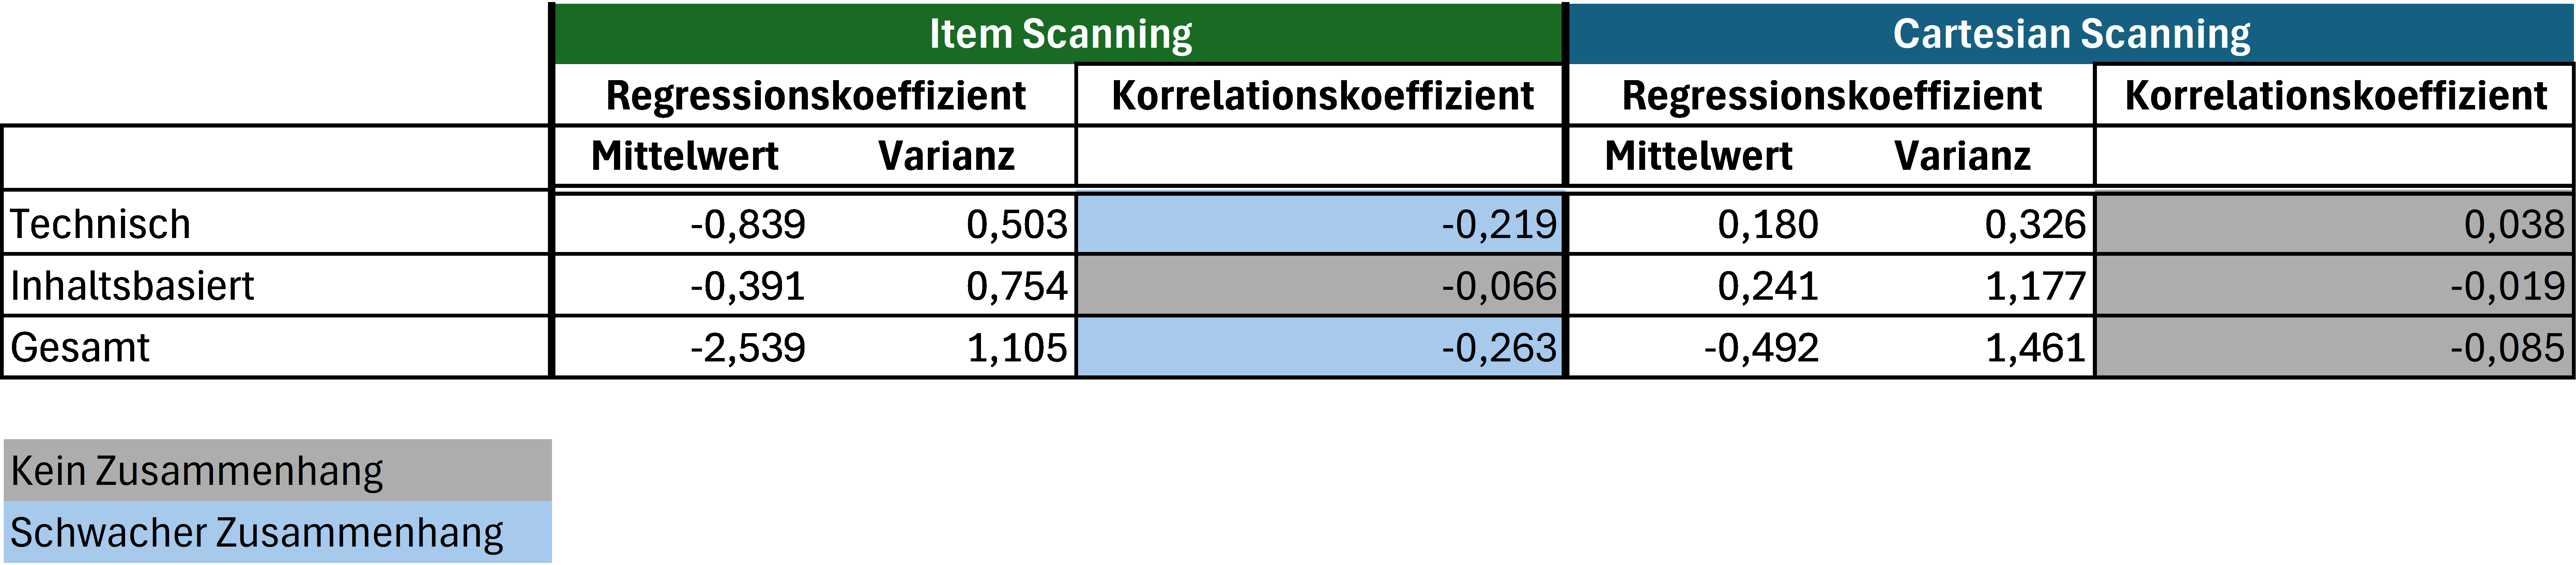
\includegraphics[width=0.95\textwidth]{images/Results/Regressionskoeffizienten-Korrelation-Table-Lernkurve-Geschwindigkeit.png}
 \caption{Regressionskoeffizienten Lernkurve}
 \label{fig:RegressionskoeffizientenTable}
\end{figure}

\subsection{Fehler und leere Eingaben}

\begin{figure}[tbh]
 \centering
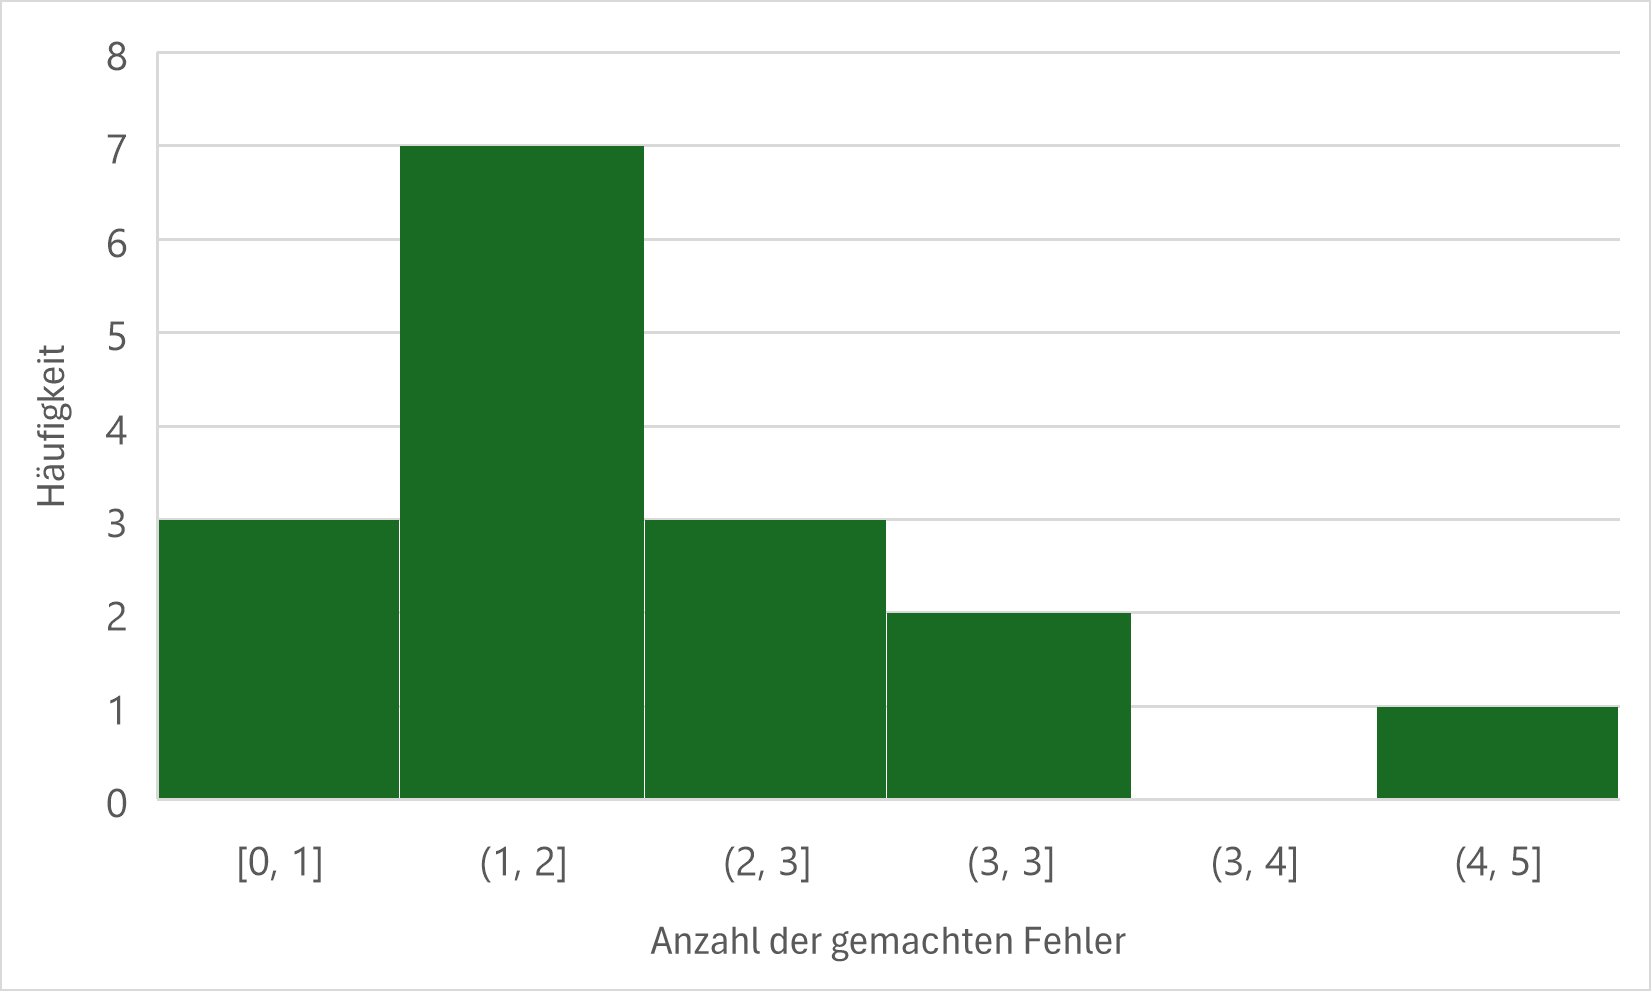
\includegraphics{images/Results/Histogramm-Anzahl-Fehler-technisch-item.png}
 \caption{Anzahl Fehler Item Technisch}
 \label{fig:anzahlFehlerItemTechnisch}
\end{figure}

\begin{figure}[tbh]
 \centering
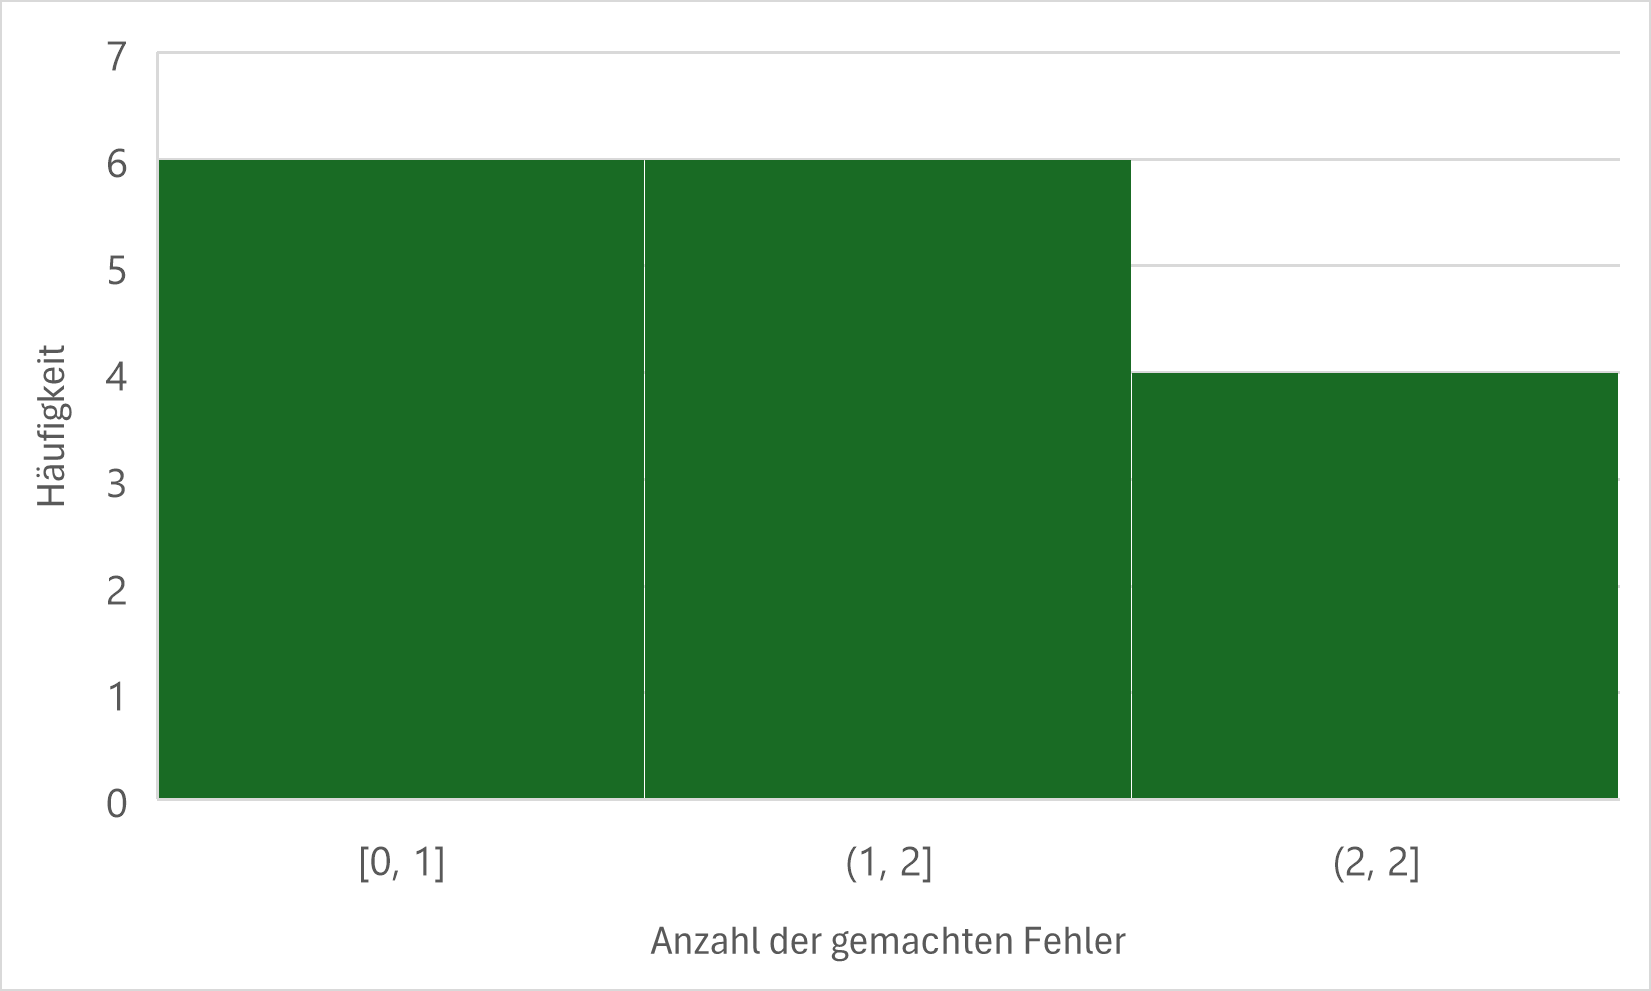
\includegraphics{images/Results/Histogramm-Anzahl-Fehler-inhalt-item.png}
 \caption{Anzahl Fehler Item Inhalt}
 \label{fig:anzahlFehlerItemInhalt}
\end{figure}

\begin{figure}[tbh]
 \centering
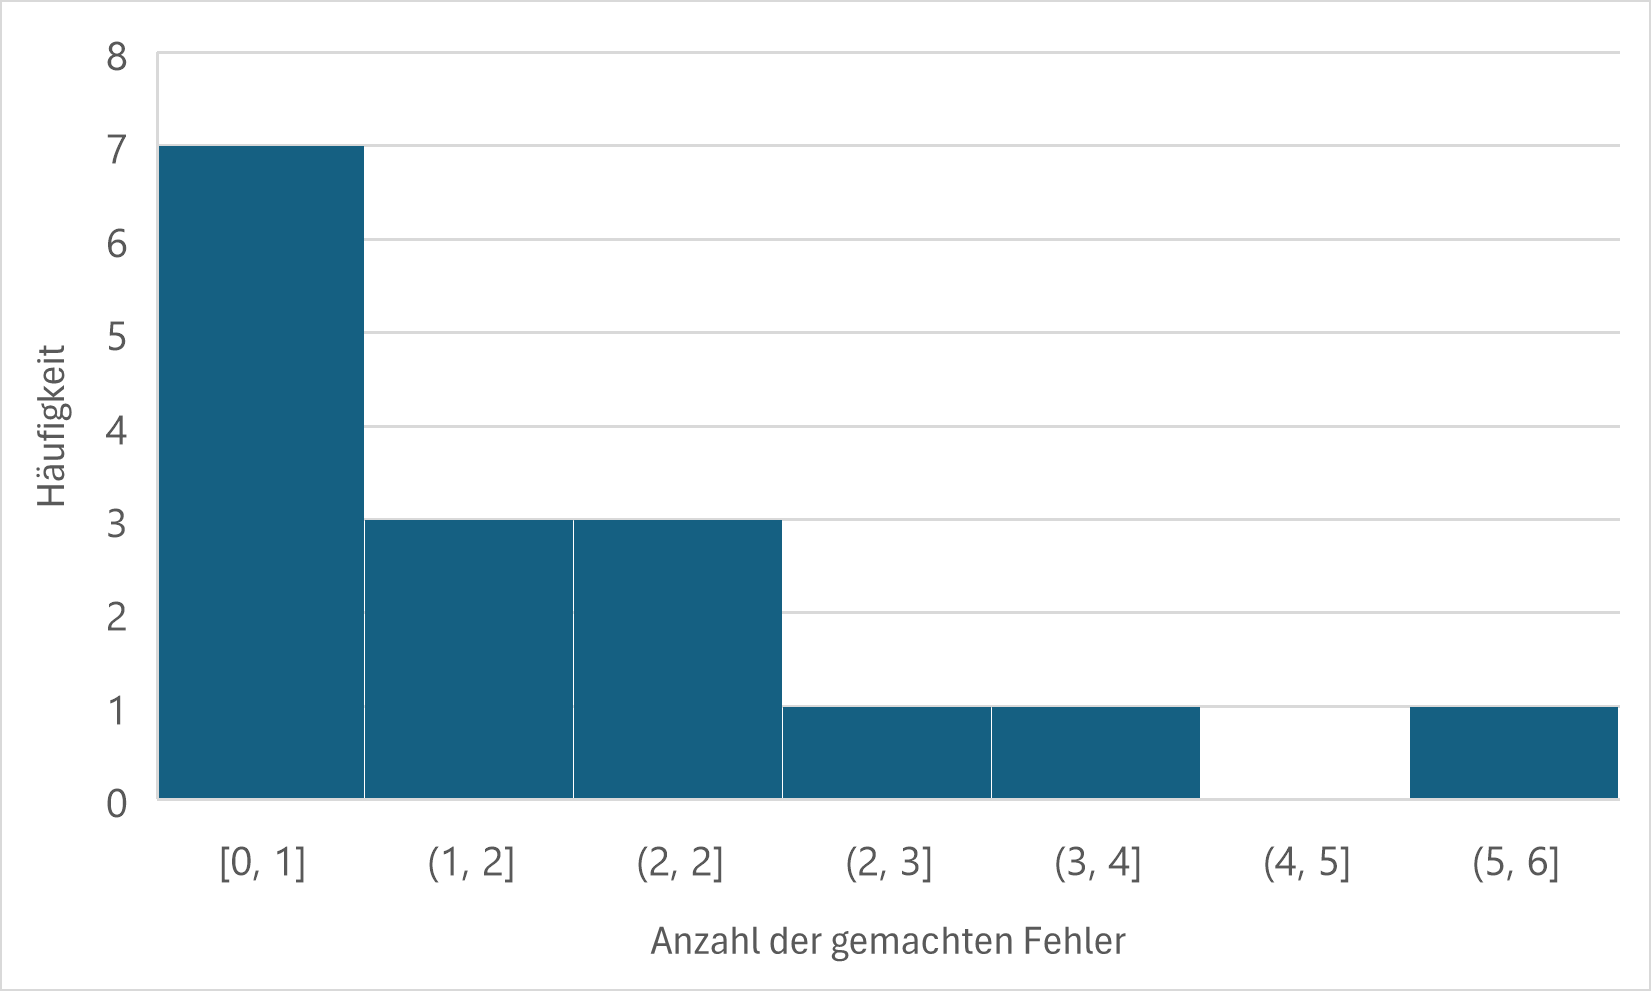
\includegraphics{images/Results/Histogramm-Anzahl-Fehler-technisch-cartesian.png}
 \caption{Anzahl Fehler Cartesian Technisch}
 \label{fig:anzahlFehlerCartesianTechnisch}
\end{figure}

\begin{figure}[tbh]
 \centering
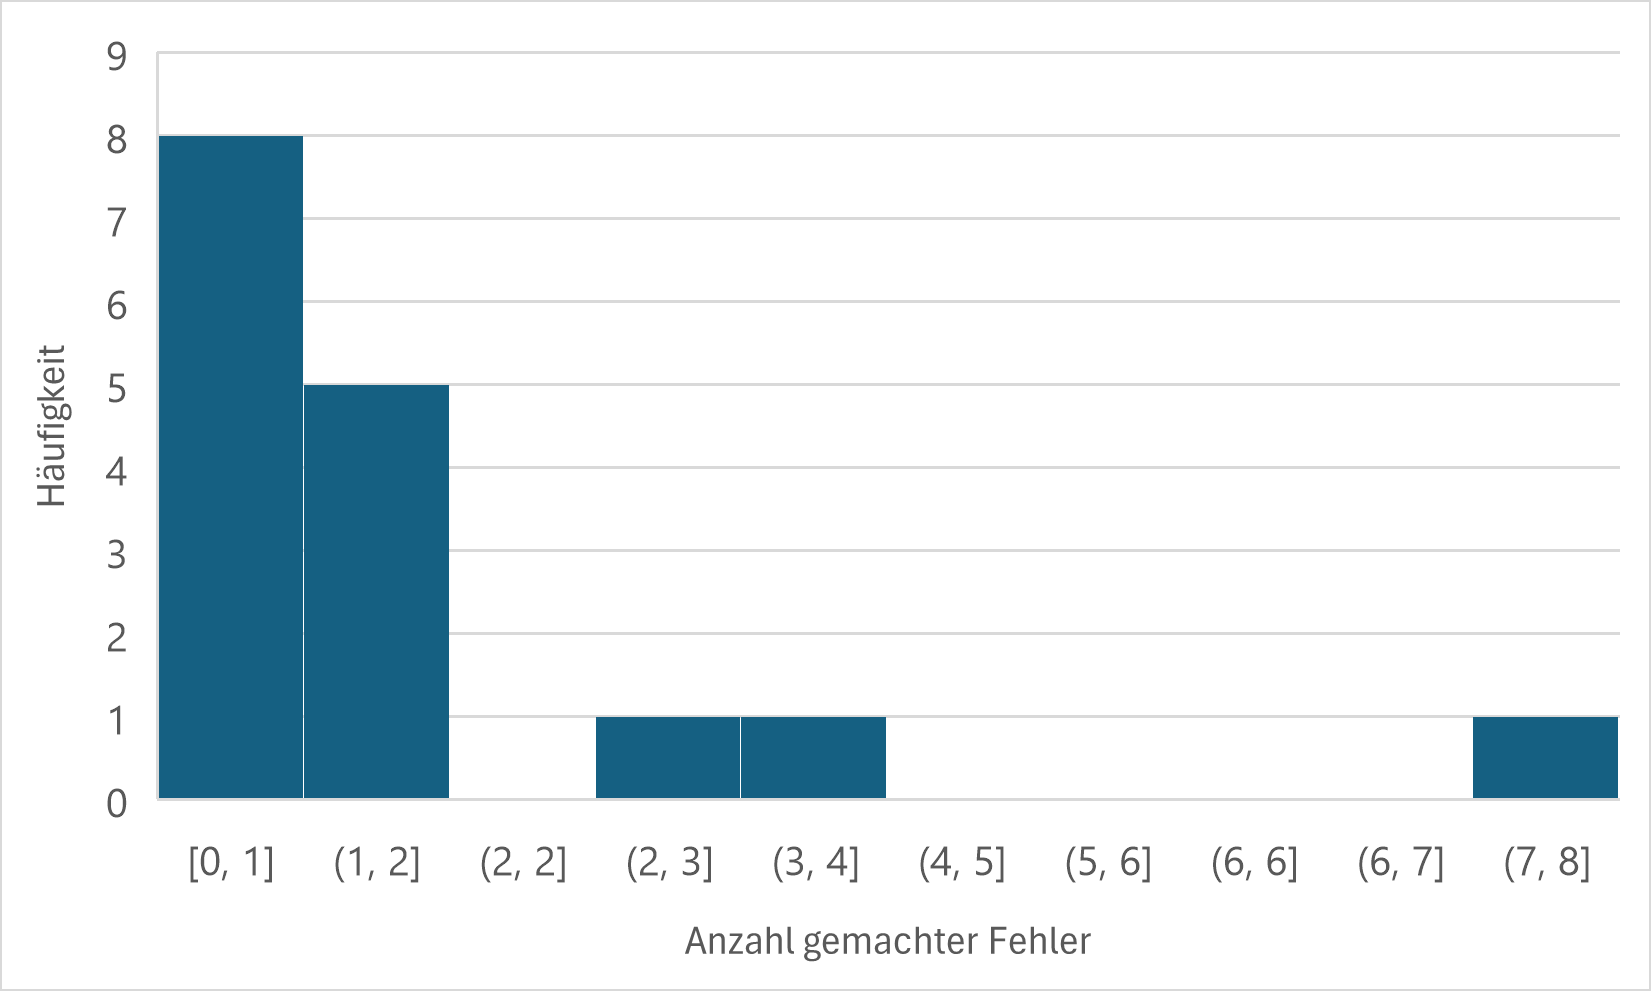
\includegraphics{images/Results/Histogramm-Anzahl-Fehler-inhalt-cartesian.png}
 \caption{Anzahl Fehler Cartesian Inhalt}
 \label{fig:anzahlFehlerCartesianInhalt}
\end{figure}

\begin{figure}[tbh]
 \centering
\includegraphics{images/Results/Gründe-Fehler-Item.png}
 \caption{Gründe für Fehler Item Scanning}
 \label{fig:gründeFehlerItem}
\end{figure}

\begin{figure}[tbh]
 \centering
\includegraphics[width=0.95\textwidth]{images/Results/Gründe-Fehler-Cartesian.png}
 \caption{Gründe für Fehler Cartesian Scanning}
 \label{fig:gründeFehlerCartesian}
\end{figure}


\subsection{Korrelationen}

\begin{figure}[tbh]
    \centering
   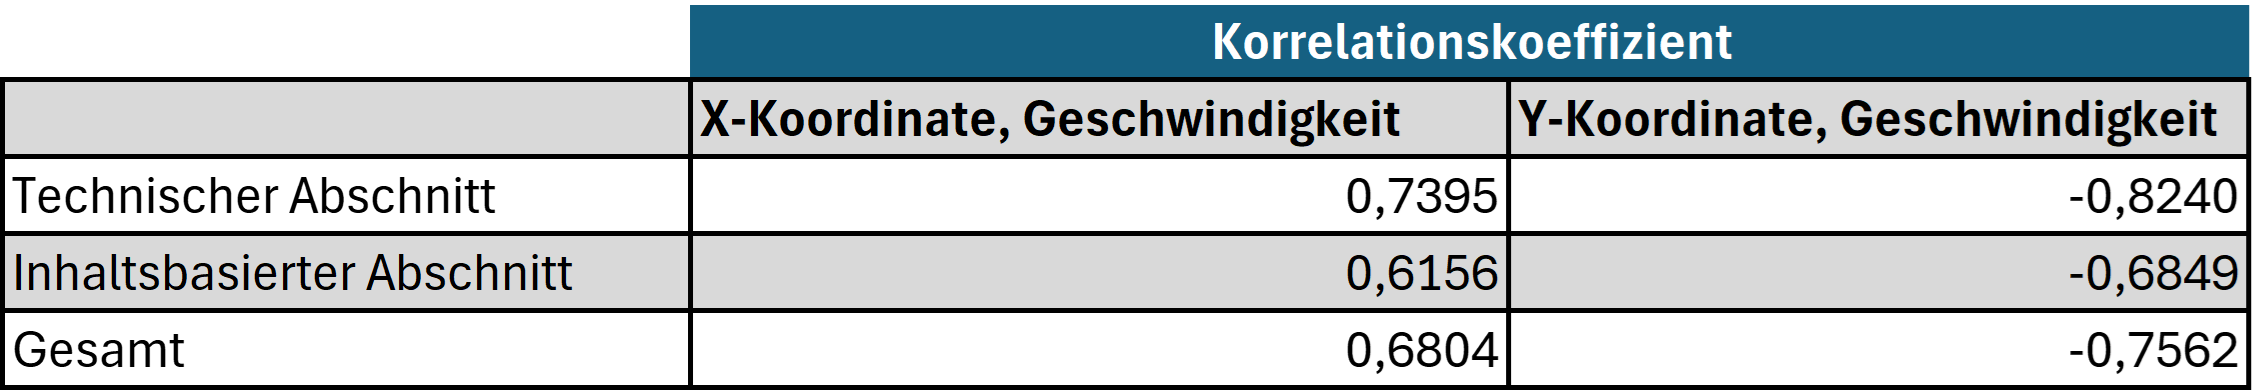
\includegraphics[width=0.95\textwidth]{images/Results/Korrelation-Position-Geschwindigkeit-Table.png}
    \caption{Zusammenhang Postion des Objekts im Sichtfeld und Selektionsgeschwindigkeit}
    \label{fig:tableKorrPosGeschwindigkeit}
   \end{figure}

   \begin{figure}[tbh]
    \centering
   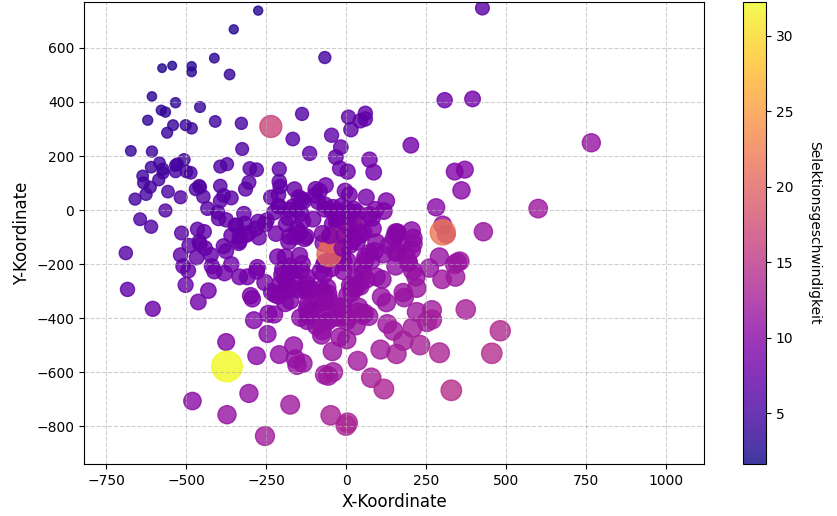
\includegraphics[width=0.95\textwidth]{images/Results/bubbleplot-inhalt.png}
    \caption{Zusammenhang Postion des Objekts im Sichtfeld und Selektionsgeschwindigkeit Inhaltsbasierter Abschnitt}
    \label{fig:bubbleKorrPosGeschwindigkeitInhalt}
   \end{figure}

   \begin{figure}[tbh]
    \centering
   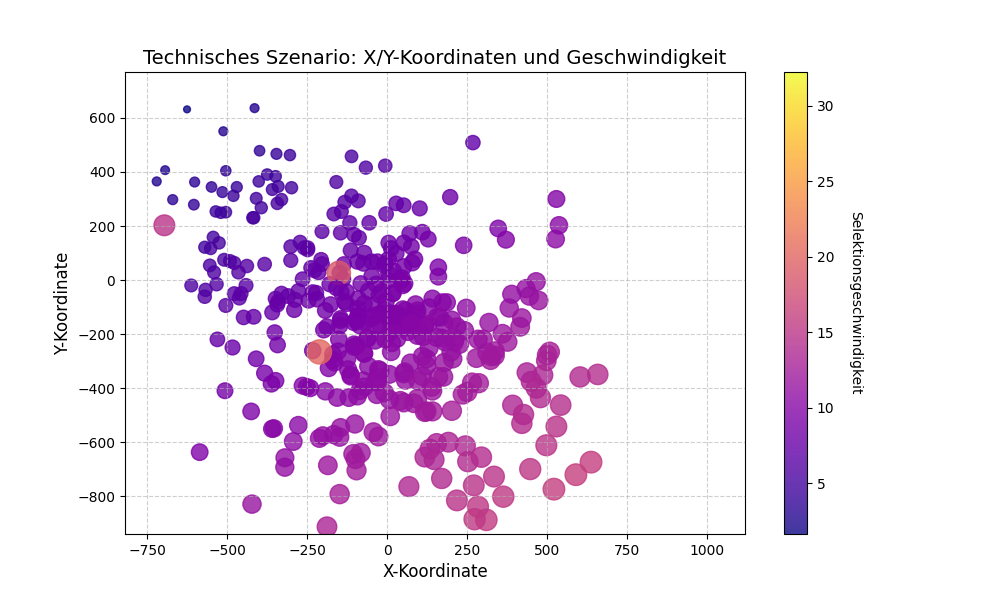
\includegraphics[width=0.95\textwidth]{images/Results/bubbleplot-technisch.png}
    \caption{Zusammenhang Postion des Objekts im Sichtfeld und Selektionsgeschwindigkeit Technischer Abschnitt}
    \label{fig:bubbleKorrPosGeschwindigkeitTechnisch}
   \end{figure}

   \begin{figure}[tbh]
    \centering
   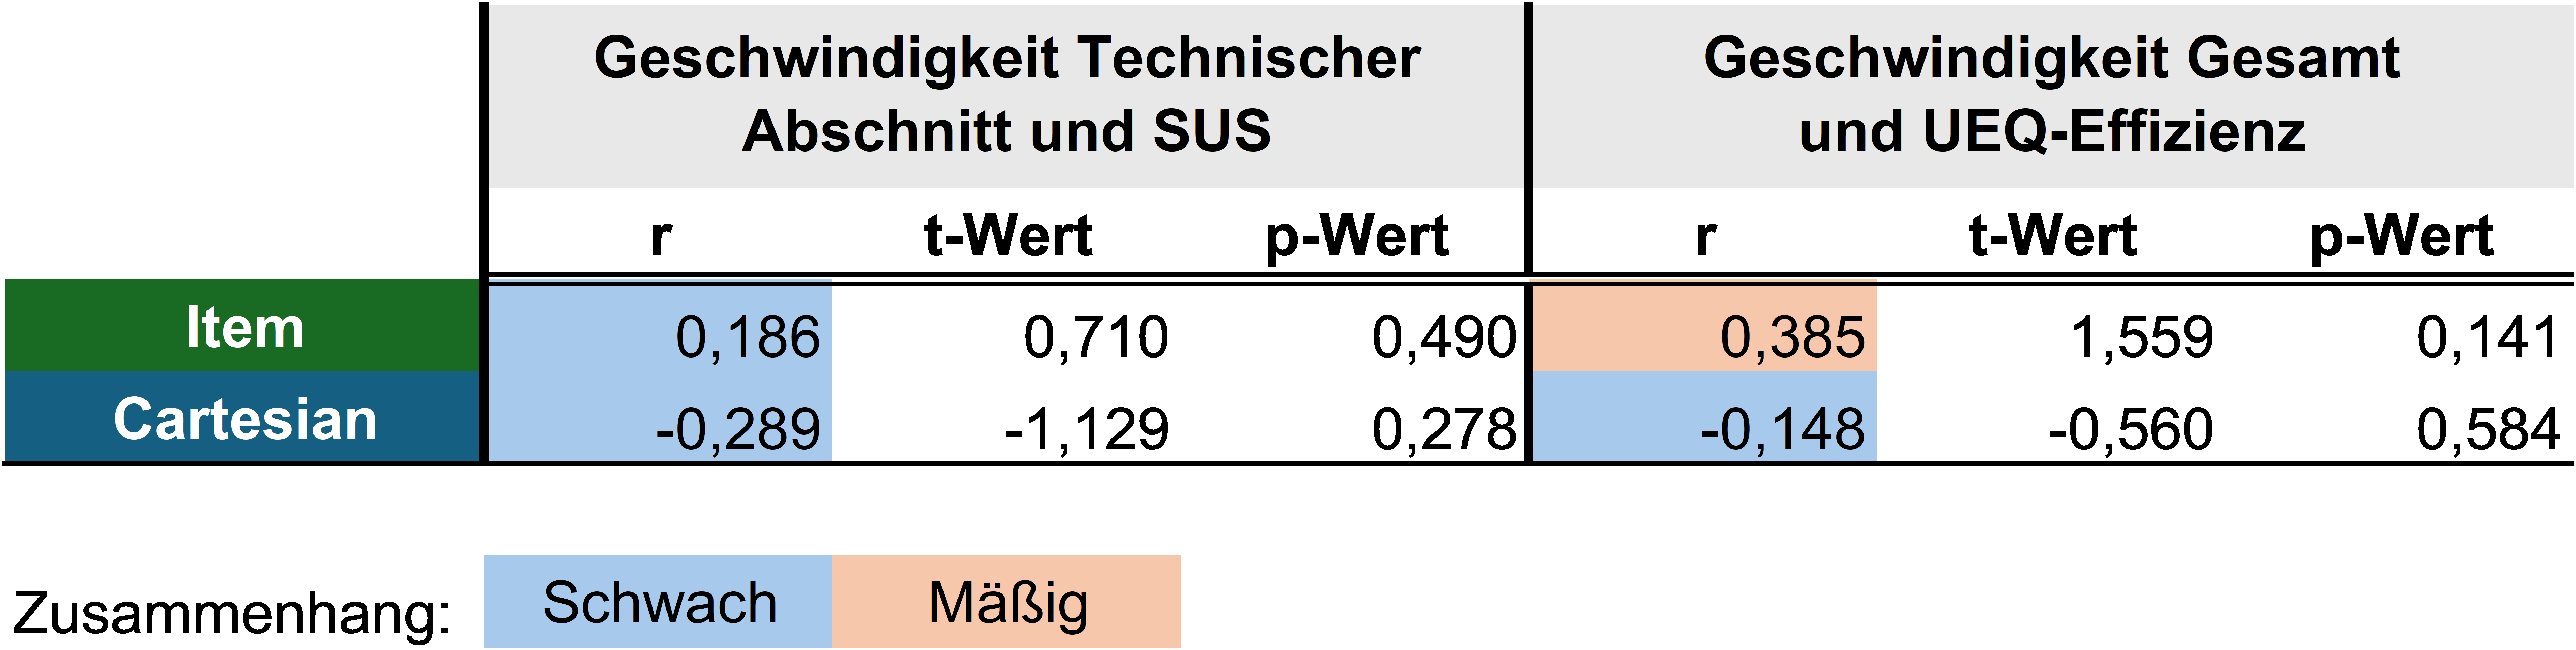
\includegraphics[width=0.95\textwidth]{images/Results/Korrelationen-Rest.png}
    \caption{Zusammenhang Interaktionsgeschwindigkeit und Usability/UX}
    \label{fig:TableKorrelationen}
   \end{figure}

\subsection{Feedback/Anmerkungen/Beobachtungen}



